\documentclass[11pt]{mimosis}
\synctex=1

% \PassOptionsToClass{14pt}{scrbook}
\usepackage{metalogo}

\usepackage{textcomp}
\usepackage{gensymb}

\usepackage[pass]{geometry}

%%%%%%%%%%%%%%%%%%%%%%%%%%%%%%%%%%%%%%%%%%%%%%%%%%%%%%%%%%%%%%%%%%%%%%%%
% Some of my favorite personal adjustments
%%%%%%%%%%%%%%%%%%%%%%%%%%%%%%%%%%%%%%%%%%%%%%%%%%%%%%%%%%%%%%%%%%%%%%%%
%
% These are the adjustments that I consider necessary for typesetting
% a nice thesis. However, they are *not* included in the template, as
% I do not want to force you to use them.

% This ensures that I am able to typeset bold font in table while still aligning the numbers
% correctly.
\usepackage{etoolbox}

\usepackage[binary-units=true]{siunitx}
\DeclareSIUnit\px{px}

\sisetup{%
  detect-all           = true,
  detect-family        = true,
  detect-mode          = true,
  detect-shape         = true,
  detect-weight        = true,
  detect-inline-weight = math,
}

%%%%%%%%%%%%%%%%%%%%%%%%%%%%%%%%%%%%%%%%%%%%%%%%%%%%%%%%%%%%%%%%%%%%%%%%
% Hyperlinks & bookmarks
%%%%%%%%%%%%%%%%%%%%%%%%%%%%%%%%%%%%%%%%%%%%%%%%%%%%%%%%%%%%%%%%%%%%%%%%

\usepackage[%
  colorlinks = true,
  citecolor  = BrickRed,
  linkcolor  = BrickRed,
  urlcolor   = BrickRed,
  % pdftex,
  pdfauthor={Jan Straub},
  pdftitle={Reflections on the correlation between the tendency to procrastinate and the likelihood to be awarded a doctoral degree},
  % pdfsubject={The Subject},
  % pdfkeywords={Some Keywords},
  % pdfproducer={Latex with hyperref, or other system},
  % pdfcreator={pdflatex, or other tool}
  ]{hyperref}

\usepackage{bookmark}


%%%%%%%%%%%%%%%%%%%%%%%%%%%%%%%%%%%%%%%%%%%%%%%%%%%%%%%%%%%%%%%%%%%%%%%%
% Bibliography
%%%%%%%%%%%%%%%%%%%%%%%%%%%%%%%%%%%%%%%%%%%%%%%%%%%%%%%%%%%%%%%%%%%%%%%%
%
% I like the bibliography to be extremely plain, showing only a numeric
% identifier and citing everything in simple brackets. The first names,
% if present, will be initialized. DOIs and URLs will be preserved.

\usepackage[%
  autocite      = plain,
  backend       = biber,
  doi           = false,
  url           = true,
  giveninits    = true,
  hyperref      = true,
  maxbibnames   = 99,
  maxcitenames  = 99,
  sortcites     = true,
  style         = alphabetic,
  citestyle     = alphabetic,
  maxalphanames = 4,           % max number of authors before it becomes [First+12]
  backref       = true,
  ]{biblatex}


%%%%%%%%%%%%%%%%%%%%%%%%%%%%%%%%%%%%%%%%%%%%%%%%%%%%%%%%%%%%%%%%%%%%%%%%
% Some adjustments to make the bibliography more clean
%%%%%%%%%%%%%%%%%%%%%%%%%%%%%%%%%%%%%%%%%%%%%%%%%%%%%%%%%%%%%%%%%%%%%%%%
%
% The subsequent commands do the following:
%  - Removing the month field from the bibliography
%  - Fixing the Oxford commma
%  - Suppress the "in" for journal articles
%  - Remove the parentheses of the year in an article
%  - Delimit volume and issue of an article by a colon ":" instead of
%    a dot ""
%  - Use commas to separate the location of publishers from their name
%  - Remove the abbreviation for technical reports
%  - Display the label of bibliographic entries without brackets in the
%    bibliography
%  - Ensure that DOIs are followed by a non-breakable space
%  - Use hair spaces between initials of authors
%  - Make the font size of citations smaller
%  - Fixing ordinal numbers (1st, 2nd, 3rd, and so) on by using
%    superscripts

% Remove the month field from the bibliography. It does not serve a good
% purpose, I guess. And often, it cannot be used because the journals
% have some crazy issue policies.
\AtEveryBibitem{\clearfield{month}}
\AtEveryCitekey{\clearfield{month}}

% Fixing the Oxford comma. Not sure whether this is the proper solution.
% More information is available under [1] and [2].
%
% [1] http://tex.stackexchange.com/questions/97712/biblatex-apa-style-is-missing-a-comma-in-the-references-why
% [2] http://tex.stackexchange.com/questions/44048/use-et-al-in-biblatex-custom-style
%
\AtBeginBibliography{%
  \renewcommand*{\finalnamedelim}{%
    \ifthenelse{\value{listcount} > 2}{%
      \addcomma
      \addspace
      \bibstring{and}%
    }{%
      \addspace
      \bibstring{and}%
    }
  }
}

% Suppress "in" for journal articles. This is unnecessary in my opinion
% because the journal title is typeset in italics anyway.
\renewbibmacro{in:}{%
  \ifentrytype{article}
  {%
  }%
  % else
  {%
    \printtext{\bibstring{in}\intitlepunct}%
  }%
}

% Remove the parentheses for the year in an article. This removes a lot
% of undesired parentheses in the bibliography, thereby improving the
% readability. Moreover, it makes the look of the bibliography more
% consistent.
\renewbibmacro*{issue+date}{%
  \setunit{\addcomma\space}
    \iffieldundef{issue}
      {\usebibmacro{date}}
      {\printfield{issue}%
       \setunit*{\addspace}%
       \usebibmacro{date}}%
  \newunit}

% Delimit the volume and the number of an article by a colon instead of
% by a dot, which I consider to be more readable.
\renewbibmacro*{volume+number+eid}{%
  \printfield{volume}%
  \setunit*{\addcolon}%
  \printfield{number}%
  \setunit{\addcomma\space}%
  \printfield{eid}%
}

% Do not use a colon for the publisher location. Instead, connect
% publisher, location, and date via commas.
\renewbibmacro*{publisher+location+date}{%
  \printlist{publisher}%
  \setunit*{\addcomma\space}%
  \printlist{location}%
  \setunit*{\addcomma\space}%
  \usebibmacro{date}%
  \newunit%
}

% Ditto for other entry types.
\renewbibmacro*{organization+location+date}{%
  \printlist{location}%
  \setunit*{\addcomma\space}%
  \printlist{organization}%
  \setunit*{\addcomma\space}%
  \usebibmacro{date}%
  \newunit%
}

% Do not abbreviate "technical report".
\DefineBibliographyStrings{english}{%
  techreport = {technical report},
}

% Display the label of a bibliographic entry in bare style, without any
% brackets. I like this more than the default.
%
% Note that this is *really* the proper and official way of doing this.
\DeclareFieldFormat{labelnumberwidth}{#1\adddot}

% Ensure that DOIs are followed by a non-breakable space.
\DeclareFieldFormat{doi}{%
  \mkbibacro{DOI}\addcolon\addnbspace
    \ifhyperref
      {\href{http://dx.doi.org/#1}{\nolinkurl{#1}}}
      %
      {\nolinkurl{#1}}
}

% Use proper hair spaces between initials as suggested by Bringhurst and
% others.
\renewcommand*\bibinitdelim {\addnbthinspace}
\renewcommand*\bibnamedelima{\addnbthinspace}
\renewcommand*\bibnamedelimb{\addnbthinspace}
\renewcommand*\bibnamedelimi{\addnbthinspace}

% Make the font size of citations smaller. Depending on your selected
% font, you might not need this.
\renewcommand*{\citesetup}{%
  \biburlsetup
  \small
}

% \DeclareLanguageMapping{british}{bibliography-correct-ordinals}
% \DeclareLanguageMapping{english}{bibliography-correct-ordinals}
\bibliography{Thesis}

%%%%%%%%%%%%%%%%%%%%%%%%%%%%%%%%%%%%%%%%%%%%%%%%%%%%%%%%%%%%%%%%%%%%%%%%
% Fonts
%%%%%%%%%%%%%%%%%%%%%%%%%%%%%%%%%%%%%%%%%%%%%%%%%%%%%%%%%%%%%%%%%%%%%%%%

\ifxetexorluatex
  %\setmainfont{Minion Pro}
  \usepackage{microtype}
\else
  %\usepackage[osf,lining]{ebgaramond}  
  \usepackage[scale=0.7]{sourcecodepro}  
\fi






\usepackage{mathpazo}
\usepackage{lettrine}

\usepackage{makeidx}
\makeindex



% \newacronym[description={Principal component analysis}]{PCA}{PCA}{principal component analysis}
% \newacronym                                            {SNF}{SNF}{Smith normal form}
% \newacronym[description={Topological data analysis}]   {TDA}{TDA}{topological data analysis}

% \makeindex
% \makeglossaries

%%%%%%%%%%%%%%%%%%%%%%%%%%%%%%%%%%%%%%%%%%%%%%%%%%%%%%%%%%%%%%%%%%%%%%%%
% Incipit
%%%%%%%%%%%%%%%%%%%%%%%%%%%%%%%%%%%%%%%%%%%%%%%%%%%%%%%%%%%%%%%%%%%%%%%%
 
\usepackage{mathtools}
\usepackage{amssymb}
\usepackage{siunitx}
\usepackage{xcolor}
\usepackage{todonotes}
\usepackage{soul}
\usepackage{algorithm}
\usepackage{algpseudocode}
\usepackage{blindtext}

% Corrects \autoref{}: chapter -> Chapter, section -> Section, subsection -> Section
\addto\extrasenglish{%
  \renewcommand{\chapterautorefname}{Chapter}%
  \renewcommand{\sectionautorefname}{Section}%
  \renewcommand{\subsectionautorefname}{Section}%
}

\begin{document}

\frontmatter
  %!TEX root = ../Thesis.tex

\begin{titlepage}
  \centering % Center all text
  \vspace*{\baselineskip} % White space at the top of the page

  %\rule{\textwidth}{1.6pt}\vspace*{-\baselineskip}\vspace*{2pt} % Thick horizontal line
  %\rule{\textwidth}{0.4pt}\\[1.0\baselineskip] % Thin horizontal line

  {\huge Visualization of Heat Waves}\\[0.2\baselineskip] % Title

  %\rule{\textwidth}{0.4pt}\vspace*{-\baselineskip}\vspace{3.2pt} % Thin horizontal line
  %\rule{\textwidth}{1.6pt}\\ % Thick horizontal line

  \vspace*{\baselineskip}

  {\Large Bachelor's Thesis\\[\baselineskip]} % Tagline(s) or further description
  \vspace*{\baselineskip}

  {\LARGE Jan Michael Straub\\[\baselineskip]} % Editor list  

  \vspace*{\baselineskip} % Whitespace between location/year and editors

  Supervisor\\
  {\large  Prof.\,Dr.\,Filip Sadlo\\[\baselineskip]} % Editor list

  \vfil

  Heidelberg,  \today \par % Location and year

  \vspace*{\baselineskip}

  {\itshape Faculty of Mathematics and Computer Science\par} % Editor affiliation
  {\itshape Heidelberg University\par} % Editor affiliation
\end{titlepage}

\cleardoublepage

  % %!TEX root = ../Thesis.tex

\selectlanguage{english}

\begin{titlepage}
  \begin{center}
    \textsc{\huge Dissertation}
                \vskip 1cm
                \begin{large}
                  submitted to the\\[0.50cm]
                  \begin{Large}
                    \textsc{Combined Faculty for the\\Natural Sciences and Mathematics}\\[0.50cm]
                  \end{Large}
                  of\\[0.50cm]
                  \begin{Large}
                    \textsc{Heidelberg University, Germany}\\[0.50cm]
                  \end{Large}
                  for the degree of \\[0.5cm] 
                  Doctor of Natural Sciences
                \end{large}
    %
    \vfill
    %
    \begin{large}
                  put forward by\\[0.5cm]
                  \begin{LARGE}
                    \textbf{Guybrush Threepwood}, M.Sc.
                  \end{LARGE}\\[0.5cm]
                  born in Ankh-Morpork, Discworld
    \end{large}
    %
    \vskip 2cm
    %
    \begin{small}
      Heidelberg\\
      Marchtember 2033
    \end{small}
  \end{center}
\end{titlepage}

\selectlanguage{english}

\begin{titlepage}
  %
  \phantom{}
  \vfill 
  %
  \begin{center}
    \begin{singlespace*}
      \begin{Huge}
          Reflections on the correlation between the tendency to procrastinate and the likelihood to be awarded a doctoral degree\par
      \end{Huge}
      %
      \vskip 0.25cm
      \emph{by}
      \vskip 0.25cm
      %
      \textsc{Guybrush Threepwood}\par
    \end{singlespace*}
  \end{center}
  %
  \vfill
  %
  \begin{singlespace*}
    Advisor:            Prof.\,Dr.\,Filip Sadlo \\[.5cm]
    Oral examination: \rule{4cm}{0.15mm}
  \end{singlespace*}
\end{titlepage}

\newpage
\null
\thispagestyle{empty}
\newpage
  % for PhD thesis
  \pagestyle{empty}
  %!TEX root = ../Thesis.tex

\section*{Declaration of Authorship}

I hereby declare that the thesis submitted is my own unaided work. All direct or indirect sources used are acknowledged as references. The principles and recommendations \enquote{Verantwortung in der Wissenschaft} of Heidelberg University have been followed.
\vspace{5cm}\\
\noindent\rule[0.5ex]{8em}{0.5pt} \hfill \rule[0.5ex]{10em}{0.5pt}\\
\noindent Jan Straub \hfill Heidelberg, date and signature  % remove for PhD thesis
  %!TEX root = ../Thesis.tex
%%%%%%%%%%%%%%%%%%%%%%%%%%%%%%%%%%%%%%%%%%%%%%%%%%%%%%%%%%%%%%%%%%%%%%%%
\begin{center}
  \textsc{Abstract}
\end{center}
\noindent

In this thesis, we presented a novel edge bundling technique based on a Physarium approximation of a Steiner tree. Here we use the Steiner tree as a routing structure for graph paths. The resulting drawings consist of densely bundled graphs that reduce node-edge overlaps and make it easier to get an overview of the graph data.

For the Physarium calculation, we utilize the network Poisson equation to simulate a liquid flow inside the graph network, which enables us to cut nodes and edges, if the conductivity in an edge gets too low. Cutting edges shrinks the network until just a Steiner tree is left. To optimize the process, we multithreaded the calculation and found optimal iteration bounds that still deliver a satisfactory approximation result.
To visualize the initial network paths, we route them via the Steiner tree and visualize them by utilizing B\'{e}zier curves.

The outcomes enhance readability and make spotting areas of interest more straightforward. We further evaluate our algorithm by calculating the quality metrics: ink reduction, distortion, and ambiguity. We compare the results to two edge bundling approaches to classify our technique and comprehend its usefulness. We additionally discuss the constraints of our method and propose further improvements to circumvent these limitations.
%%%%%%%%%%%%%%%%%%%%%%%%%%%%%%%%%%%%%%%%%%%%%%%%%%%%%%%%%%%%%%%%%%%%%%%%

\cleardoublepage

  %!TEX root = ../Thesis.tex

\begin{center}
  \textsc{Zusammenfassung}
\end{center}
%
\selectlanguage{ngerman}
\noindent 

Diese Arbeit stellt einen neuen edge bundling Ansatz vor, welcher die Approximierung von Steinerbäumen mittels einer Physariumapproximierung durchführt. Der Steinerbaum wird dann als Struktur für das Routing von den ursprünglichen Graph Pfaden benutzt. Die resultierenden Darstellungen bestehen aus dichten Graphen, deren Knoten-Kanten Überschneidungen reduziert wurden und es dadurch einfacher ist, sich einen Überblick über die Daten zu verschaffen.

Für die Physariumapproximierung nutzten wir die Netzwerk-Poisson-Gleichung, um einen Fluss von Flüssigkeit im Graph zu simulieren. Sobald die Leitfähigkeit einer Kante zu gering wird, wird diese gelöscht. Dies führt dazu, dass der Graph sich immer weiter zusammenzieht, bis am Ende ein Steinerbaum übrigbleibt. Um den Prozess zu optimieren, haben wir für die Berechnungen Multithreading benutzt und die optimalen Iterationsgrenzen gefunden, welche trotzdem noch eine zufriedenstellende Approximation erreichen.
Um die ursprünglichen Graph Pfade darzustellen, suchen wir den besten Weg durch den Steinerbaum und stellen diesen dann mit Hilfe einer Bezierkurve dar.

Für die Evaluierung unserer Methode nutzen wir die Qualitätsmerkmale: Tintenreduzierung, Verzerrung und Mehrdeutigkeit. Die Ergebnisse vergleichen wir mit zwei anderen Ansätzen, um unseren Ansatz einordnen zu können und seinen Nutzen zu verstehen. Außerdem besprechen wir die Einschränkungen unserer Idee und schlagen möglichen Verbesserungen vor.

\selectlanguage{english}
\cleardoublepage

  \tableofcontents

\mainmatter
  \pagestyle{scrheadings}

  %!TEX root = ../Thesis.tex

%%%%%%%%%%%%%%%%%%%%%%%%%%%%%%%%%%%%%%%%%%%%%%%%%%%%%%%%%%%%%%%%%%%%%%%%
\chapter{Introduction}
%%%%%%%%%%%%%%%%%%%%%%%%%%%%%%%%%%%%%%%%%%%%%%%%%%%%%%%%%%%%%%%%%%%%%%%%

\begin{figure}[t]
  \centering
  
\includegraphics[width=0.5\linewidth]{figures/dummy}
  \caption{Do not state the obvious. Do not state the obvious. Do not state the obvious. Do not state the obvious. Do not state the obvious. Do not state the obvio.}
\end{figure}

But I must explain to you how all this mistaken \hyperref[sec:index]{idea}\index{idea} of denouncing pleasure and praising pain was born and I will give you a complete account of the system, and expound the actual teachings of the great explorer of the truth, the master-builder of human happiness. No one rejects, dislikes, or avoids pleasure itself, because it is pleasure, but because those who do not know how to pursue pleasure rationally encounter consequences that are extremely painful. Nor again is there anyone who loves or pursues or desires to obtain pain of itself, because it is pain, but because occasionally circumstances occur in which toil and pain can procure him some great pleasure. 

To take a trivial example, which of us ever undertakes laborious physical exercise, except to obtain some advantage from it? But who has any right to find fault with a man who chooses to enjoy a pleasure that has no annoying consequences, or one who avoids a pain that produces no resultant pleasure? On the other hand, we denounce with righteous indignation and dislike men who are so beguiled and demoralized by the charms of pleasure of the moment, so blinded by desire, that they cannot foresee the pain and trouble that are bound to ensue; and equal blame belongs to those who fail in their duty through weakness of will, which is the same as saying through shrinking from toil and pain. These cases are perfectly simple and easy to distinguish. In a free hour, when our power of choice is untrammelled and when nothing prevents our being able to do what we like best, every pleasure is to be welcomed and every pain avoided. But in certain circumstances and owing to the claims of duty or the obligations of business it will frequently occur that pleasures have to be repudiated and annoyances accepted. The wise man therefore always holds in these matters to this principle of selection: he rejects pleasures to secure other greater pleasures, or else he endures pains to avoid worse pains. 

But I must explain to you how all this mistaken \hyperref[sec:index]{idea}\index{idea} of denouncing pleasure and praising pain was born and I will give you a complete account of the system, and expound the actual teachings of the great explorer of the truth, the master-builder of human happiness. No one rejects, dislikes, or avoids pleasure itself, because it is pleasure, but because those who do not know how to pursue pleasure rationally encounter consequences that are extremely painful. Nor again is there anyone who loves or pursues or desires to obtain pain of itself, because it is pain, but because occasionally circumstances occur in which toil and pain can procure him some great pleasure. To take a trivial example, which of us ever undertakes laborious physical exercise, except to obtain some advantage from it? But who has any right to find fault with a man who chooses to enjoy a pleasure that has no annoying consequences, or one who avoids a pain that produces no resultant pleasure? On the other hand, we denounce with righteous indignation and dislike men who are so beguiled and demoralized by the charms of pleasure of the moment, so blinded by desire, that they cannot foresee the pain and trouble that are bound to ensue; and equal blame belongs to those who fail in their duty through weakness of will, which is the same as saying through shrinking from toil and pain. These cases are perfectly simple and easy to distinguish. In a free hour, when our power of choice is untrammelled and when nothing prevents our being able to do what we like best, every pleasure is to be welcomed and every pain avoided. But in certain circumstances and owing to the claims of duty or the obligations of business it will frequently occur that pleasures have to be repudiated and annoyances accepted. The wise man therefore always holds in these matters to this principle of selection: he rejects pleasures to secure other greater pleasures, or else he endures pains to avoid worse pains. But I must explain to you how all this mistaken \hyperref[sec:index]{idea}\index{idea} of denouncing pleasure and praising pain was born and I will give you a complete account of the system, and expound the actual teachings of the great explorer of the truth, the master-builder of human happiness. No one rejects, dislikes, or avoids pleasure itself, because it is pleasure, but because those who do not know how to pursue pleasure rationally encounter consequences that are extremely painful.

Nor again is there anyone who loves or pursues or desires to obtain pain of itself, because it is pain, but because occasionally circumstances occur in which toil and pain can procure him some great pleasure. To take a trivial example, which of us ever undertakes laborious physical exercise, except to obtain some advantage from it? But who has any right to find fault with a man who chooses to enjoy a pleasure that has no annoying consequences, or one who avoids a pain that produces no resultant pleasure? On the other hand, we denounce with righteous indignation and dislike men who are so beguiled and demoralized by the charms of pleasure of the moment, so blinded by desire, that they cannot foresee the pain and trouble that are bound to ensue; and equal blame belongs to those who fail in their duty through weakness of will, which is the same as saying through shrinking from toil and pain. These cases are perfectly simple and easy to distinguish. 

In a free hour, when our power of choice is untrammelled and when nothing prevents our being able to do what we like best, every pleasure is to be welcomed and every pain avoided. But in certain circumstances and owing to the claims of duty or the obligations of business it will frequently occur that pleasures have to be repudiated and annoyances accepted. The wise man therefore always holds in these matters to this principle of selection: he rejects pleasures to secure other greater pleasures, or else he endures pains to avoid worse pains. But I must explain to you how all this mistaken \hyperref[sec:index]{idea}\index{idea} of denouncing pleasure and praising pain was born and I will give you a complete account of the system, and expound the actual teachings of the great explorer of the truth, the master-builder of human happiness. No one rejects, dislikes, or avoids pleasure itself, because it is pleasure, but because those who do not know how to pursue pleasure rationally encounter consequences that are extremely painful. Nor again is there anyone who loves or pursues or desires to obtain pain of itself, because it is pain, but because occasionally circumstances occur in which toil and pain can procure him some great pleasure. To take a trivial example, which of us ever undertakes laborious physical exercise, except to obtain some advantage from it? But who has any right to find fault with a man who chooses to enjoy a pleasure that has no annoying consequences, or one who avoids a pain that produces no resultant pleasure? On the other hand, we denounce with righteous indignation and dislike men who are so beguiled and demoralized by the charms of pleasure of the moment, so blinded by desire, that they cannot foresee the pain and trouble that are bound to ensue; and equal blame belongs to those who fail in their duty through weakness of will, which is the same as saying through shrinking from toil and pain. 
  %!TEX root = ../Thesis.tex

%%%%%%%%%%%%%%%%%%%%%%%%%%%%%%%%%%%%%%%%%%%%%%%%%%%%%%%%%%%%%%%%%%%%%%%%
\chapter{Related Work}
\label{sec:relatedWork}
%%%%%%%%%%%%%%%%%%%%%%%%%%%%%%%%%%%%%%%%%%%%%%%%%%%%%%%%%%%%%%%%%%%%%%%%

\Blindtext[12] Do not forget to use references~\cite{Hanser2019energy} like done here~\cite{Hofmann2019dependentVectors} to enable the bibliography~\cite{Jung2017tumble, Sagrista2019GaiaSky, Sdeo2018fullerene, Zheng2019equivalence}.
  %!TEX root = ../Thesis.tex

%%%%%%%%%%%%%%%%%%%%%%%%%%%%%%%%%%%%%%%%%%%%%%%%%%%%%%%%%%%%%%%%%%%%%%%%
\chapter{Fundamentals}
\label{sec:fundamentals}
As the section above already focused on the slime mold and Steiner trees, and the subsequent chapters heavily rely on a firm grasp of those topics, it is vital to lay down some fundamentals before going further. Furthermore, it is paramount to understand the basics of graphs and edge bundling, the fundamental concepts of the mathematical definition of Physarium Polycephalum, and the terminology. 

%%%%%%%%%%%%%%%%%%%%%%%%%%%%%%%%%%%%%%%%%%%%%%%%%%%%%%%%%%%%%%%%%%%%%%%%
\section{Graphs}
\label{sec:graphs}

For this thesis, we define a graph as a structure that links unmovable points with lines to allow a representation of relations between objects. In mathematical terms, a graph is defined as $G = (V, E)$, where $V$ are the vertices or nodes and $E$ the edges where $E \subseteq \{\{x, y\} | x, y \in V \text{ and } x \neq y\}$. A graph is either directed or undirected. If a graph is directed, the edges between vertices have a direction; otherwise, they are bidirectional \cite{noauthor_graph_2022}. Important to note is that for calculation purposes, graphs in this thesis are discretized into a grid, which is also a graph. The difference between our grid graph and a regular graph is that all nodes that are not original graph nodes can be moved and deleted.
%%%%%%%%%%%%%%%%%%%%%%%%%%%%%%%%%%%%%%%%%%%%%%%%%%%%%%%%%%%%%%%%%%%%%%%%

\newpage

\begin{figure}[H]
    \centering
    \begin{subfigure}{0.20\linewidth}
        \centering
        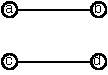
\includegraphics[width=0.9\linewidth]{figures/amb/amb_0.pdf}
        \caption{}
        \label{fig:amb_0}
    \end{subfigure}
    \begin{subfigure}{0.20\linewidth}
        \centering
        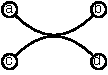
\includegraphics[width=0.9\linewidth]{figures/amb/amb_1.pdf}
        \caption{}
        \label{fig:amb_1}
    \end{subfigure}
    \begin{subfigure}{0.29\linewidth}
        \centering
        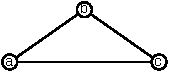
\includegraphics[width=\linewidth]{figures/amb/amb_2.pdf}
        \caption{}
        \label{fig:amb_2}
    \end{subfigure}
    \begin{subfigure}{0.29\linewidth}
        \centering
        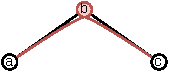
\includegraphics[width=\linewidth]{figures/amb/amb_3.pdf}
        \caption{}
        \label{fig:amb_3}
    \end{subfigure}
    \caption{Graphs \subref{fig:amb_0} and \subref{fig:amb_1} demonstrate the independent edge ambiguity, as in \subref{fig:amb_0} the start and end point of each edge is clearly defined and distinguishable. Still, in the bundled layout in \subref{fig:amb_1}, there is no way to distinguish what connections were made in the original graph. The path endpoint ambiguity is shown in \subref{fig:amb_2} and \subref{fig:amb_3}. As \subref{fig:amb_3} shows, it might be possible to bundle an edge too strong, which could intersect with a node. Images \subref{fig:amb_0} and \subref{fig:amb_1} from \cite{Straub2022}.}
    \label{fig:amb}
\end{figure}

%%%%%%%%%%%%%%%%%%%%%%%%%%%%%%%%%%%%%%%%%%%%%%%%%%%%%%%%%%%%%%%%%%%%%%%%
\section{Bundling Techniques}
\label{sec:bundling_techniques}

Bundling describes a technique that reduces the number of edges and makes a graph visualization more appealing. These results can be archived by bundling paths with similar properties using structures for bundling paths, cluster paths by simulating physical properties, and many more, as seen in \autoref{sec:relatedWork}. This process can reveal high-level patterns and make the graph easier to comprehend.
These graph manipulations also have their drawbacks, as briefly mentioned above. With bundling, the chances for independent edge ambiguities, as shown in \autoref{fig:amb_0} and \autoref{fig:amb_1}, increase, which means that two or more edges get so close to one another that they are no longer distinguishable, and the readability is severely reduced. Bundling approaches can also have path endpoint ambiguities, \autoref{fig:amb_2} and \autoref{fig:amb_3}, such as node-edge overlaps; they occur when the bundling is so firm that the bundled path crosses a node. It is then no longer possible to discern whether the path connects to this node. The last significant ambiguity is edge crossings, as a shallow crossing angle leads to falsely perceived path connections \cite{wallinger_edge-path_2022}.
%%%%%%%%%%%%%%%%%%%%%%%%%%%%%%%%%%%%%%%%%%%%%%%%%%%%%%%%%%%%%%%%%%%%%%%%

\begin{figure}[H]
    \centering
    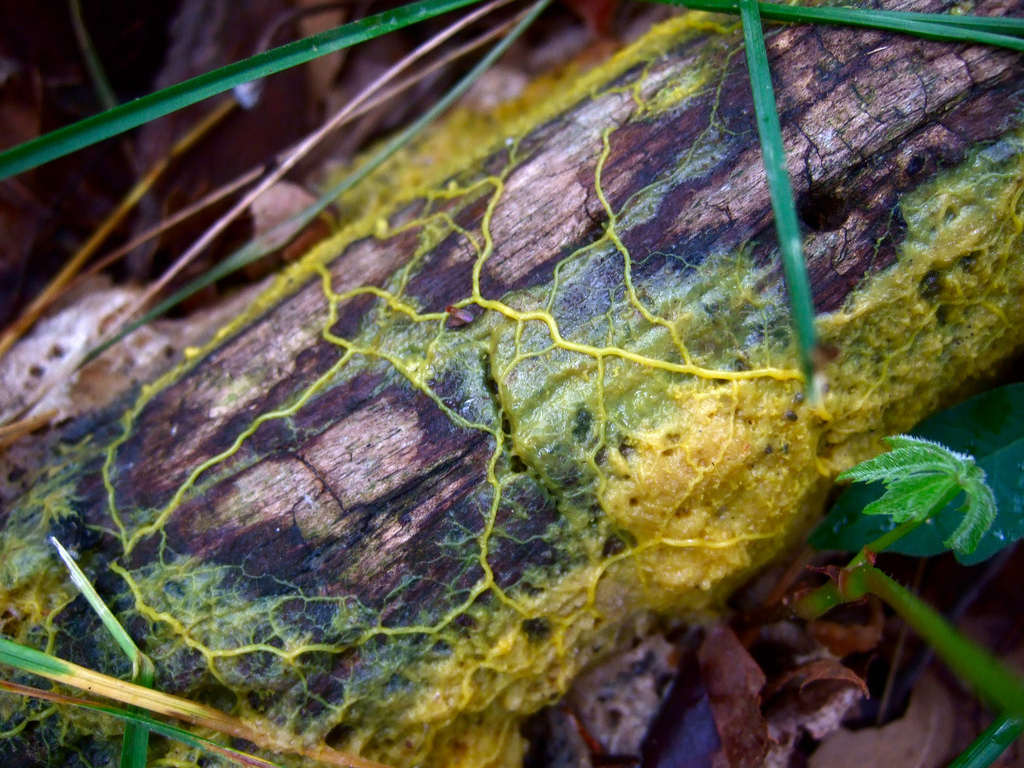
\includegraphics[width=0.75\linewidth]{figures/Physarum_polycephalum_plasmodium.jpg}
    \caption{P. Polycephalum plasmodium (yellow) on tree bark. Easy to spot are the protoplasmic tubes that connect different food sources and parts of the organism \cite{physarium_picture}. These tubes and the processes that control them are the goals of our Physarium approximation algorithm.}
    \label{fig:physarium_picture}
\end{figure}

%%%%%%%%%%%%%%%%%%%%%%%%%%%%%%%%%%%%%%%%%%%%%%%%%%%%%%%%%%%%%%%%%%%%%%%%
\section{Physarium Polycephalum}
\label{sec:polycephalum}

Physarium Polycephalum is a unicellular true slime mold organism that lives on rotten wood and mushrooms, where it can reach a size of multiple square meters. It is, therefore, one of the only cells humans can see with their own eyes and is one of the oldest organisms on earth \cite{jabr_how_2012}. It has a life cycle of four stages, but this thesis will focus only on the plasmodium stage in \autoref{fig:physarium_picture}. In 2000, Nakagaki et al. \cite{nakagaki_maze-solving_2000, nakagaki_path_2001} used this behavior to prove that the slime mold can find the shortest path in a maze. Ten years later, Tero et al. showed that Physarium could solve complicated grids efficiently as the slime mold traced the Tokyo rail system \cite{tero_rules_2010}. The slime mold can also solve the minimal Steiner tree problem in graphs, as Zhang et al. proved \cite{zhang_improved_2014}.

Physarium can archive these results by the ability to move, as the organism constantly searches for new food sources. As mentioned above, this stage is called the plasmodium stage. In this stage, protoplasmic tubes connect to different food sources and circulate nutrients and chemical signals throughout the organism. This tube network can rearrange its structure and continuously contracts to the minimal length, which is the most efficient transport method. The organism finds new food sources through the ability to identify different chemical gradients by using a net-like search structure and following the path with the most robust one. The organism archives mobility by the forward and backward motion of the cytoplasm inside the tubes. This motion is also known as shuttle streaming. Two factors decide the tube efficiency: The first one is the tube diameter which increases or decreases according to the flow. A high flow increases tube diameter, and a low flow rate leads to a decrease. The second one is the length of the tube. A longer tube accelerates the reduction of the diameter \cite{adamatzky2016advances, tero_mathematical_2007}. 

Mathematically this behavior can be described by the pressure difference in two connected vertices and the resulting Poiseuille flow through the edge as the fluid equalizes the pressure \cite{liu_physarum_2015}. The flux in an edge $e_{i,j}$ is described by $Q_{i,j}$, where $D_{i,j}$ denotes the conductivity of $e_{i,j}$, $p_{i}$ and $p_{j}$ are the pressures at $v_i$ and $v_j$, $\xi$ is the viscosity coefficient, and $C_{ij}$ the edge cost. 

\begin{equation}
    \label{eqn:flux}
    Q_{i,j} = \frac{\pi r^{4}_{ij}(p_i-p_j)}{8 \xi C_{ij}} = \frac{D_{i,j}}{C_{i,j}}(p_i-p_j)
\end{equation}

\begin{equation}
    \label{eqn:conductivity_eqn}
    D_{i, j} = \frac{\pi r_{I,j}^{4}}{8\xi}
\end{equation}

After calculating the flux, one vertex is selected as a flow source $v_s$.
With the network Poisson equation \autoref{eqn:poisson_eqn}, it is possible to calculate the pressures in each vertex. 

\begin{equation}
    \label{eqn:poisson_eqn}
    \sum\limits_{i \in V{j}} \frac{D_{i,j}}{C_{ij}}(p_i-p_j) = \begin{cases}
        I_0, \text{ if } j = \text{source}; \\
        -I_0, \text{ if } j = \text{sink}; \\
        0, \text{ otherwise}
    \end{cases}
\end{equation}

However, besides finding efficient paths in networks, Physarium Polycephalum has other interesting properties that researchers can use. For example, the plasmodium stage creates Voronoi diagrams as it expands \cite{shirakawa_simultaneous_2009}; it can learn to anticipate certain events and react before they arrive, and it knows which nutrients it needs for the fastest growth rate \cite{jabr_how_2012}. It can be used as an electric wire to connect components, as Lu and Lopes demonstrated in their study \cite{lu_integrating_2022}.
%%%%%%%%%%%%%%%%%%%%%%%%%%%%%%%%%%%%%%%%%%%%%%%%%%%%%%%%%%%%%%%%%%%%%%%%

%%%%%%%%%%%%%%%%%%%%%%%%%%%%%%%%%%%%%%%%%%%%%%%%%%%%%%%%%%%%%%%%%%%%%%%%
\section{Physarium Network Terms}
\label{sec:network_terms}

As graphs in this thesis are used to simulate fluid networks, it is essential to introduce some specific terms used throughout it. Starting with terminals $T$ where $T \subseteq V$. Terminals are normal nodes in the grid graph at the position of an original graph node. Non-terminal nodes are only created for the calculation of the Steiner points. Other terms that we use in the context of this thesis are sink and source nodes. A source node injects an initial flow $I_0$ into the network. A sink node serves as an outlet for the flow, as in fluid dynamics, the flow conservation has to apply \cite{black_flow_2004}. A Physarium network can have multiple sink or source nodes. How fast the fluid can flow through the network is determined by the conductivity value of the tube, which is dependent on the tube's radius and the fluid's viscosity. The flux is directly related to conductivity, as it describes the amount of fluid flowing through the tube.
%%%%%%%%%%%%%%%%%%%%%%%%%%%%%%%%%%%%%%%%%%%%%%%%%%%%%%%%%%%%%%%%%%%%%%%%

%%%%%%%%%%%%%%%%%%%%%%%%%%%%%%%%%%%%%%%%%%%%%%%%%%%%%%%%%%%%%%%%%%%%%%%%
\section{Steiner Trees}
\label{sec:steinertrees}

\begin{figure}[t]
    \centering
    \begin{subfigure}{0.35\linewidth}
        \centering
        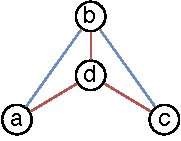
\includegraphics[width=\linewidth]{figures/spannbaum_steiner.pdf}
    \end{subfigure}
  \caption{In blue, a possible minimal spanning tree for the graph $a, b, c$ is drawn; in red, the edges for the Steiner tree, with the node $d$ as a Steiner point.}
  \label{fig:steiner_tree_example}
\end{figure}

Steiner trees, named after the Swiss mathematician Jakob Steiner, were first described in the 19th century. However, their use was limited as the calculation by hand was not feasible for larger graphs. As computers became popular, the approximation of this NP-complete problem became possible, and since then, more and more use cases have emerged. Such as the positioning of telecommunication infrastructure \cite{voss_steiner_2006}, efficiently connecting facility location \cite{eisenbrand_connected_2010}, and other related problems, such as the traveling salesman problem, can also be solved. A compendium of different Steiner tree problems can be found at \cite{Hauptmann_compendium_2015}.

The most relevant problem for this thesis is the Euclidean Steiner tree problem, where the goal is a graph where the total length of the edges is shorter than a minimal spanning tree. In mathematical terms: If $G = (V, E, c)$ is a graph where $c$ is the cost associated with each edge and $N \subseteq V$ is a set of terminals, the Steiner tree is a subgraph $T_G(N)$ of $G$ where every terminal is accessible by a path and the total length of $T_G(N)$ is minimized \cite{byrka_steiner_2013}. The difference to a minimal spanning tree is that Steiner trees can create so-called Steiner points to reduce the overall length of the graph \cite{noauthor_steiner_2022} and are therefore not restricted to the graph edges. A visually easy-to-understand example of the difference between a minimal spanning tree and a Steiner tree can be seen in \autoref{fig:steiner_tree_example}. These Steiner points always have three edge connections and an angle of 120° degrees between each edge. Every Steiner tree with $n$ terminals has a limit of $n - 2$ Steiner points; if all n terminals are leaves, the limit of Steiner points is reached. If a Steiner tree is cut into two new Steiner trees, the new trees will again be a complete Steiner tree. A complete Steiner tree is a Steiner tree with the maximal number of Steiner points. An angle below 120° degrees can not exist in a Steiner tree. Because if it existed, there would be a Steiner point such that the overall length would be smaller, and the 120° angle is given \cite{noauthor_steinerbaumproblem_2021}.
%%%%%%%%%%%%%%%%%%%%%%%%%%%%%%%%%%%%%%%%%%%%%%%%%%%%%%%%%%%%%%%%%%%%%%%%

%%%%%%%%%%%%%%%%%%%%%%%%%%%%%%%%%%%%%%%%%%%%%%%%%%%%%%%%%%%%%%%%%%%%%%%%
\section{Fermat Point}
\label{sec:fermat_point}

We use the Fermat or Torricelli point to move from a discrete to a continuous plot. The Fermat point is the point inside a triangle where the sum of distances to each vertex is minimal. This calculation requires no angles larger than 120° between the vertices. If an angle is greater than 120°, the vertex at the angle becomes the Fermat point. In the context of Steiner trees, the Fermat point has the same conditions as the Steiner point, and it is legit to use this calculation and still expect the results to be Steiner points. 

To calculate the Fermat point, we first have to calculate all angles inside the triangle and check if they are greater than 120°. $A = (x_0, y_0)$, $B = (x_1, y_1)$, $C = (x_2, y_2)$ are the vertices,  $a$, $b$, $c$ are the length of the respected edge, and $\alpha$, $\beta$, $\gamma$ are the angles that are calculated using $y$ and the secant $sec_{\delta}$.

\begin{equation}
    \label{eqn:calculate_angle}
    y = \arccos{\left(\frac{b^2 + c^2 - a^2}{2bc}\right)}
\end{equation}

\begin{equation}
    \label{eqn:calculation_secant}
    sec_{\delta} = \frac{1}{\cos \left(\delta - \frac{\pi}{6}\right)}
\end{equation}

To calculate the position of the Fermat point $F = (x_F, y_F)$, we use $(x_F,y_F)$.

\begin{equation}
    \label{eqn:fermat_position_x}
    (x_F,y_F) = \frac{A_{(x,y)} \cdot a \cdot sec_{\alpha} + B_{(x,y)} \cdot b \cdot sec_{\beta} + C_{(x,y)} \cdot c \cdot sec_{\gamma}}{sec_{\alpha} + sec_{\beta} + sec_{\gamma}}
\end{equation}
%%%%%%%%%%%%%%%%%%%%%%%%%%%%%%%%%%%%%%%%%%%%%%%%%%%%%%%%%%%%%%%%%%%%%%%%
  %!TEX root = ../Thesis.tex

%%%%%%%%%%%%%%%%%%%%%%%%%%%%%%%%%%%%%%%%%%%%%%%%%%%%%%%%%%%%%%%%%%%%%%%%
\chapter{Method}
\label{sec:method}

In this chapter, we use the concepts previously described in \autoref{sec:fundamentals} to outline how our algorithm works. It is divided into the search for the correct algorithm and the modifications that lead to our desired result. It also contains the optimization of the algorithm and the visualization of the final result.
%%%%%%%%%%%%%%%%%%%%%%%%%%%%%%%%%%%%%%%%%%%%%%%%%%%%%%%%%%%%%%%%%%%%%%%%

%%%%%%%%%%%%%%%%%%%%%%%%%%%%%%%%%%%%%%%%%%%%%%%%%%%%%%%%%%%%%%%%%%%%%%%%
\section{Motivation}
\label{sec:motivation}
The motivation for this topic stems from the challenging and intriguing idea of using a natural process to solve a computer science problem. The notion of this came as an afterthought of a seminar, in which two edge bundling papers (Winding Roads \cite{lambert_winding_2010} and Edge-Path Bundling \cite{wallinger_edge-path_2022} were discussed. The apparent problem is that Edge-Path Bundling and many other edge bundling algorithms lack a mathematical structure. This lack gave us the idea to use a Steiner tree as a base for the bundling. The Steiner tree also has other beneficial attributes to path bundling. As the tree connects all nodes with the minimal distance between them, and the Steiner points are at the Fermat points, the resulting bundle results in dramatically reduced clutter and a graph whose readability is improved as node-edge overlaps are reduced. 

Despite the existence of other, faster approximation algorithms for Steiner trees like SCIP-Jack \cite{RehfeldtKoch2023}, we decided to use a Physarium Polycephalum approximation algorithm to approximate the Steiner tree. The Physarium algorithm gives us a sound basis for further graph bundling, where we can use the calculation without needing post-processing. The faster calculation was not feasible in the scope of this work; instead, we used the Steiner tree as a routing structure for graph paths. These are ideal for edge bundling as they reduce the size of the graph to a minimum while still connecting all edges and also enable good readability. 
%%%%%%%%%%%%%%%%%%%%%%%%%%%%%%%%%%%%%%%%%%%%%%%%%%%%%%%%%%%%%%%%%%%%%%%%

%%%%%%%%%%%%%%%%%%%%%%%%%%%%%%%%%%%%%%%%%%%%%%%%%%%%%%%%%%%%%%%%%%%%%%%%
\section{Different Approaches of Calculating a Steiner Tree}
\label{sec:different_approaches}

Throughout this thesis, we tried different approaches to calculate a Steiner tree. In the following section, we want to present each method and discuss why we choose it and what benefits or drawbacks each has.

%%%%%%%%%%%%%%%%%%%%%%%%%%%%%%%%%%%%%%%%%%%%%%%%%%%%%%%%%%%%%%%%%%%%%%%%
\subsection{Agent Based Physarium Simulation}
\label{sec:agent-based_approach}

\begin{figure}[t]
    \centering
    \begin{subfigure}{0.45\linewidth}
        \centering
        \includegraphics[width=\linewidth]{figures/agent_plots/simulation_t250_1.png}
        \caption{}
        \label{fig:jeff_0}
    \end{subfigure}
    \begin{subfigure}{0.45\linewidth}
        \centering
        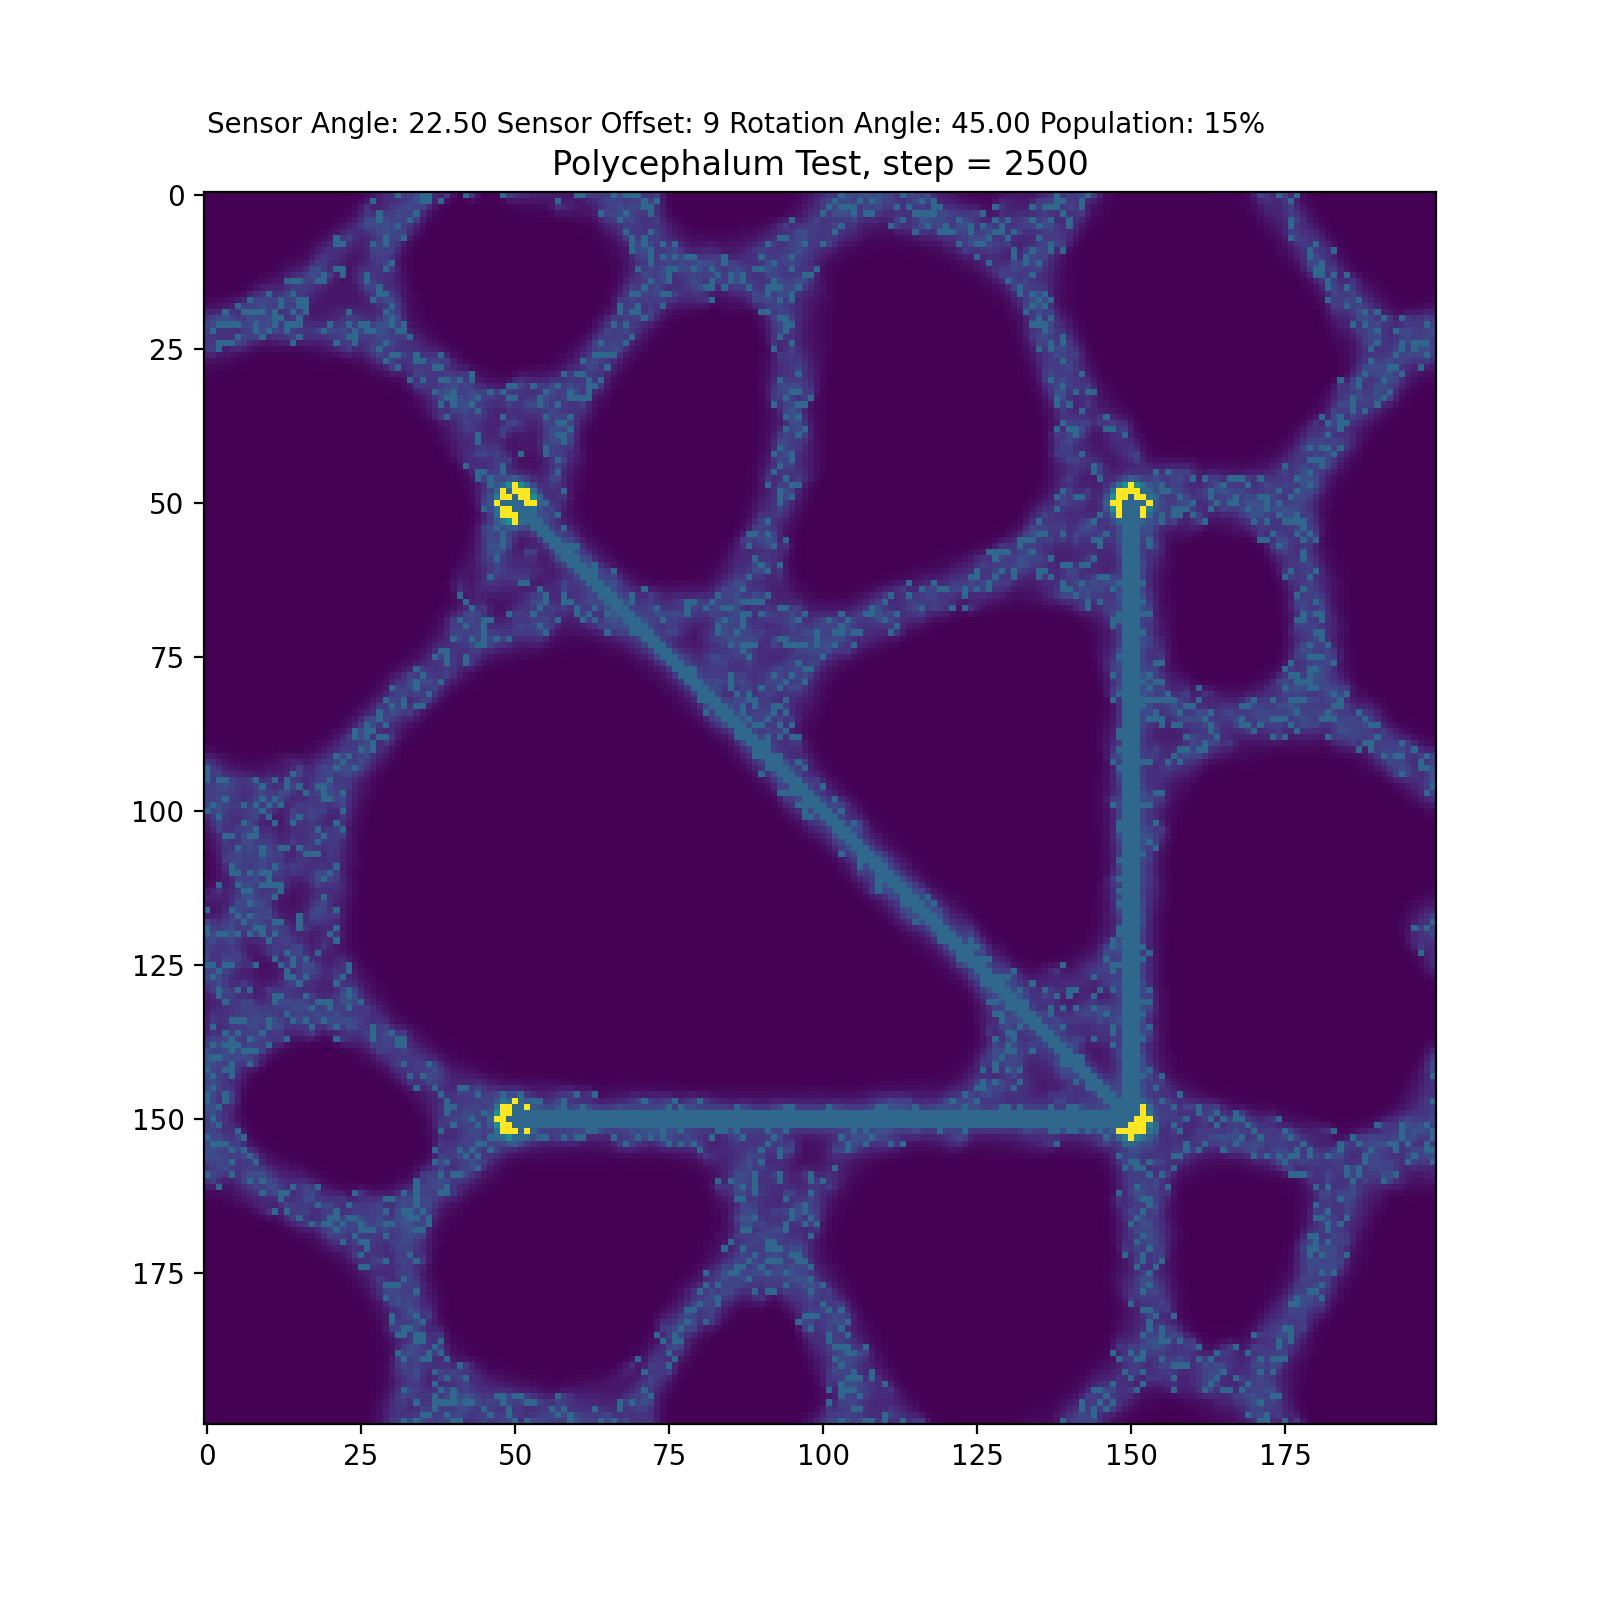
\includegraphics[width=\linewidth]{figures/agent_plots/simulation_t2499.png}
        \caption{}
        \label{fig:jeff_1}
    \end{subfigure}
  \caption{\subref{fig:jeff_0} 250 iterations with five nodes and 165 agents; \subref{fig:jeff_1} 2500 iterations with edges already present for bundling direction.}
  \label{fig:agent_plots}
\end{figure}

At first, we used an agent-based algorithm by Jones et al. \cite{jones_characteristics_2010}. The agents that are used in this approach follow two simple rules based on chemotaxis:

\begin{itemize}
    \item [1.] Deposit trail that diffuses over time
    \item [2.] Sense trails that are left behind by other agents and move in the direction in which the trail is strongest
\end{itemize}

Given enough iterations, the agents form complex patterns that merge into efficient networks. An example network can be seen in \autoref{fig:jeff_0}. We encountered two problems early on. The first was that the patterns were not stable. We tried to mitigate this problem by introducing predetermined paths for a more stable result, as seen in \autoref{fig:jeff_1}. Still, the second problem was that extracting the resulting network efficiently and retaining its accuracy was not feasible. 
%%%%%%%%%%%%%%%%%%%%%%%%%%%%%%%%%%%%%%%%%%%%%%%%%%%%%%%%%%%%%%%%%%%%%%%%

%%%%%%%%%%%%%%%%%%%%%%%%%%%%%%%%%%%%%%%%%%%%%%%%%%%%%%%%%%%%%%%%%%%%%%%%
\subsection{Biology-Inspired Steiner Tree Algorithm}
\label{sec:biology_approach}

We found a paper by Liu et al. \cite{liu_physarum_2015} for the following approach. They stimulate the cytoplasmic flow in the Polycephalum tubes by using the network Poisson equation described in \autoref{sec:physariumPolycephalum}. They discretized the graph onto a grid to find the Steiner points of a graph. The terminals then become an inflow or outflow. Each node contains a list of all combinations of inflows and outflows, and at each iteration, the conductivity and the pressure for each combination are calculated. The edge is cut from the graph if the conductivity is smaller than a threshold. For the pressure update, they use \autoref{eqn:continues_pressure_eqn}, where $p_{i,k}^t$ denotes the pressure at vertex $i$ at iteration step $t$, and $r_k$ is the sink node. 

\begingroup
\large
\begin{equation}
    \label{eqn:continues_pressure_eqn}
    p_{i,k}^{t+1} \approx \begin{cases}
        \frac{I_0 + \sum\limits_{v_j \in N_i} D_{i,j}^{i+1}(p_{i,k}^t + p_{j,k}^t)}{2 \sum\limits_{v_j \in N_i}}, \text{ for } v_i \in T \backslash \{r_k\}; \\
        0, \text{ for } v_i = r_k; \\
        \frac{\sum\limits_{v_j \in N_i} D_{i,j}^{i+1}(p_{i,k}^t + p_{j,k}^t)}{2 \sum\limits_{v_j \in N_i}}, \text{ for } v_i \notin T
    \end{cases}
\end{equation}
\endgroup

The problem with this approach was that they defined points outside the grid, calculated the edge cost concerning these points, and found the best path around them. This was no viable solution for us, as we had to find the overall shortest route in the graph independent from specific points. We also had some problems tuning the parameters to work with our approach.
%%%%%%%%%%%%%%%%%%%%%%%%%%%%%%%%%%%%%%%%%%%%%%%%%%%%%%%%%%%%%%%%%%%%%%%%

%%%%%%%%%%%%%%%%%%%%%%%%%%%%%%%%%%%%%%%%%%%%%%%%%%%%%%%%%%%%%%%%%%%%%%%%
\subsection{Node Weighted Steiner Tree Algorithm}
\label{sec:node_weighted_approach}

The third paper \cite{sun_fast_2016} takes the same approach as the second one by simulation the cytoplasmic flow with the network Poisson equation. The difference is that the node weight and the edge cost are both considered in the equation. Sun et al. used the same flux equation noted in \autoref{eqn:flux} and calculated the composite cost $C(i,j)$ for each edge. $w_i$ are the node weights, $d_i$ the degree and $M$ the maximal weight of all nodes.

\begin{equation}
    \label{eqn:composite_cost_eqn}
    C(i,j) = c_{ij} - \frac{w_i}{d_i} - \frac{w_j}{d_j} + 2M
\end{equation}

They also do not work with the pressure combination to calculate the conductivity. Instead, they use a probability equation to choose the sink node. They then sort the cost in ascending order and select a terminal using $P(i)$. $l(i)$ is the total cost of all edges connected to terminal $i$. $l(i)$ is the total cost of all edges combined.

\begin{equation}
    \label{eqn:probability_eqn}
    P(i) = \frac{l(T-i+1)}{\sum\limits_{j = 1}^Tl(j)}
\end{equation}

The pressure at each vertex is calculated using \autoref{eqn:poisson_eqn}, and the flux is calculated with \autoref{eqn:flux}. After the flux calculation, the conductivity $D_{ij}(k+1)$ needs to be updated. $\alpha_{ij}$ is a positive variable for each edge, $\mu$ a constant and the function $f$ is defined as an increasing function with $f(0) = 0$, and $f(|Q_{ij}(k)|) = \alpha |Q_{ij}(k)|$ and $\alpha$ is another positive variable.

\begin{equation}
    \label{eqn:conductivity_update_eqn}
    D_{ij}(k+1) = \alpha_{ij} \cdot [D_{ij}(k) + f(|Q_{ij}(k)|) - \mu D_{ij}(k)]
\end{equation}

Edges are cut if the conductivity is smaller than the threshold $\epsilon$. This calculation is done $K$ times in the inner iteration.

As this algorithm works with a probability equation to choose the sink node, it is not guaranteed to find the lowest-cost solution in one attempt. Therefore the authors added an outer iteration that calculates a complete network $N$ times. After each run, the total cost of the network is calculated, and if it is lower than in the last iteration, the lower-cost network is saved. 
%%%%%%%%%%%%%%%%%%%%%%%%%%%%%%%%%%%%%%%%%%%%%%%%%%%%%%%%%%%%%%%%%%%%%%%%

\newpage

%%%%%%%%%%%%%%%%%%%%%%%%%%%%%%%%%%%%%%%%%%%%%%%%%%%%%%%%%%%%%%%%%%%%%%%%
\begin{figure}[H]
    \begin{subfigure}{0.32\linewidth}
        \centering
        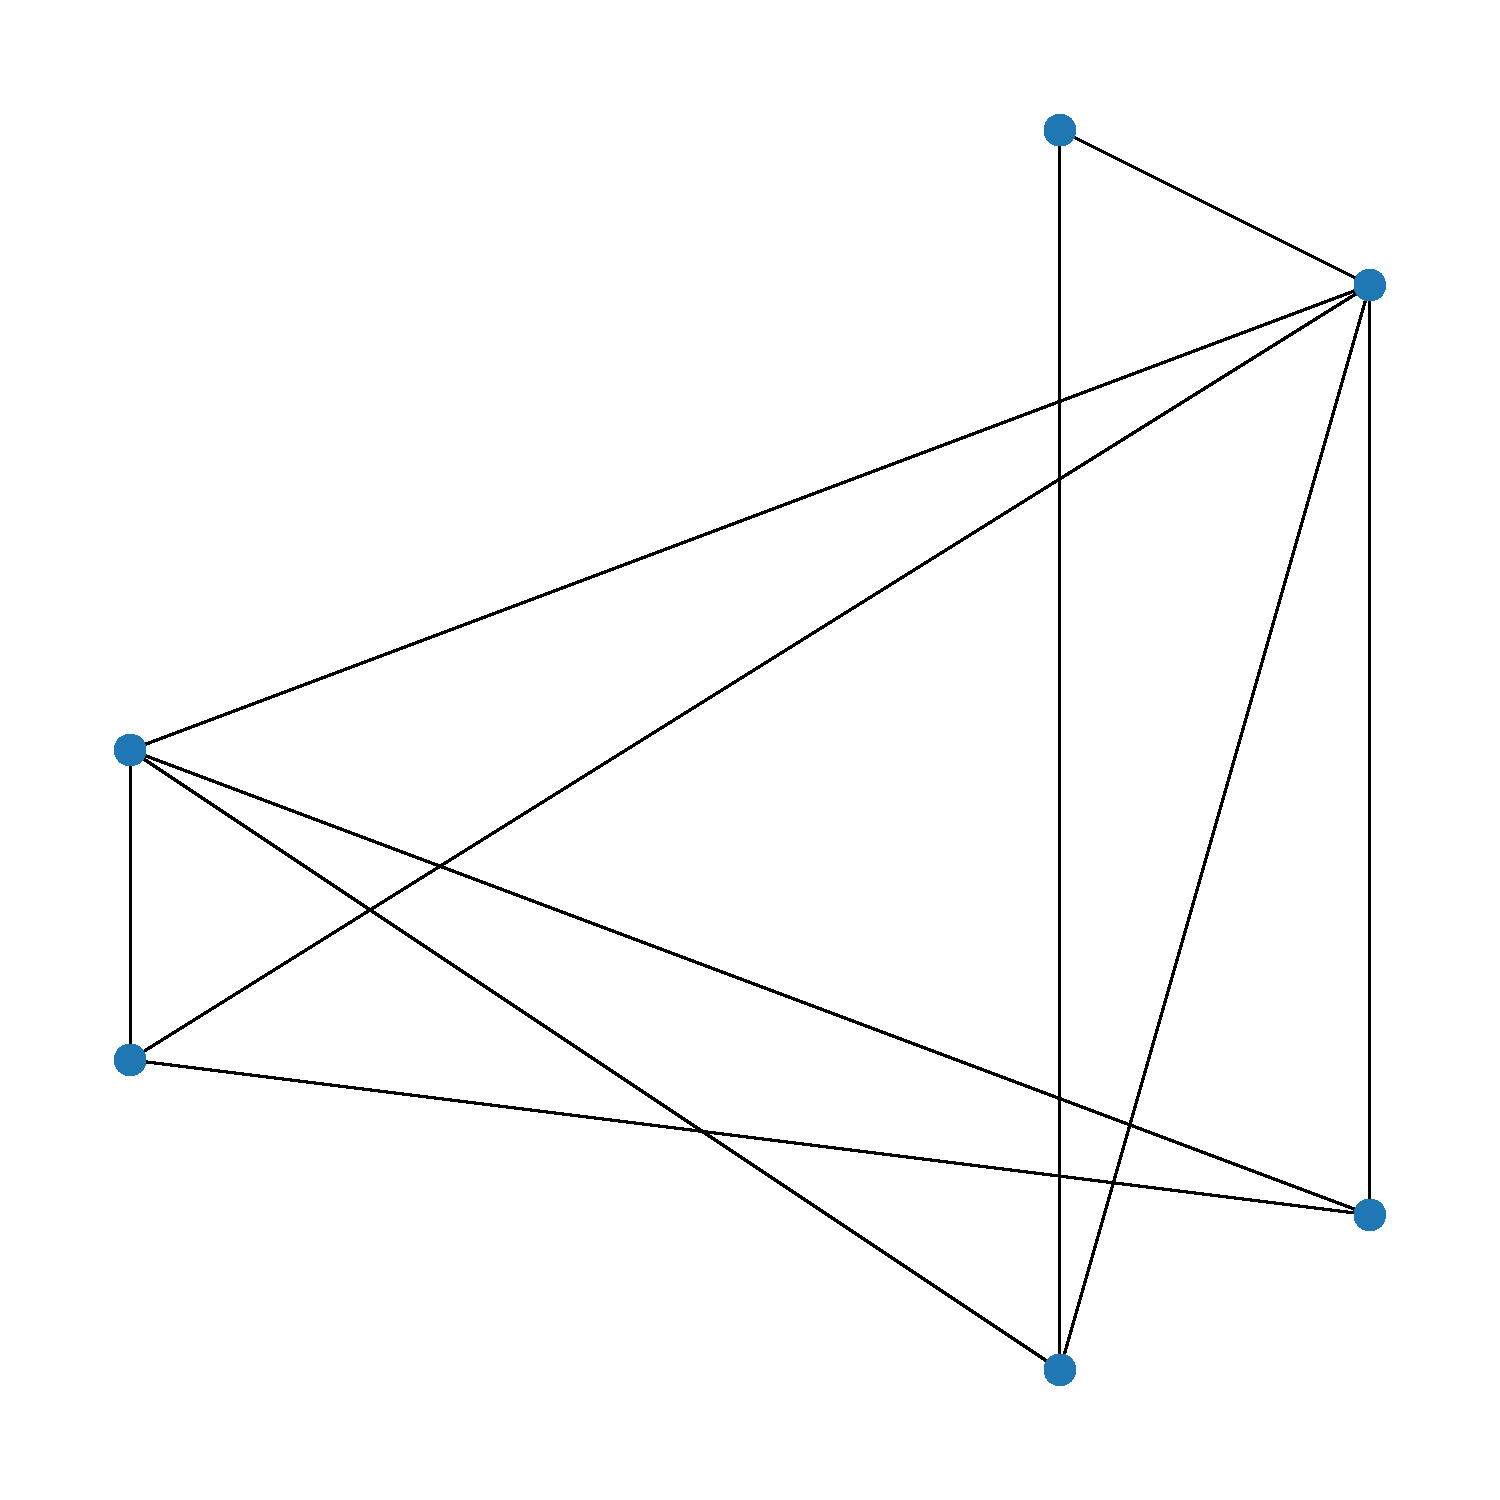
\includegraphics[width=\linewidth]{figures/algo_progress/original_default_graph.pdf}
        \caption{Straight-line graph}
        \label{fig:def_0}
    \end{subfigure}
    \begin{subfigure}{0.32\linewidth}
        \centering
        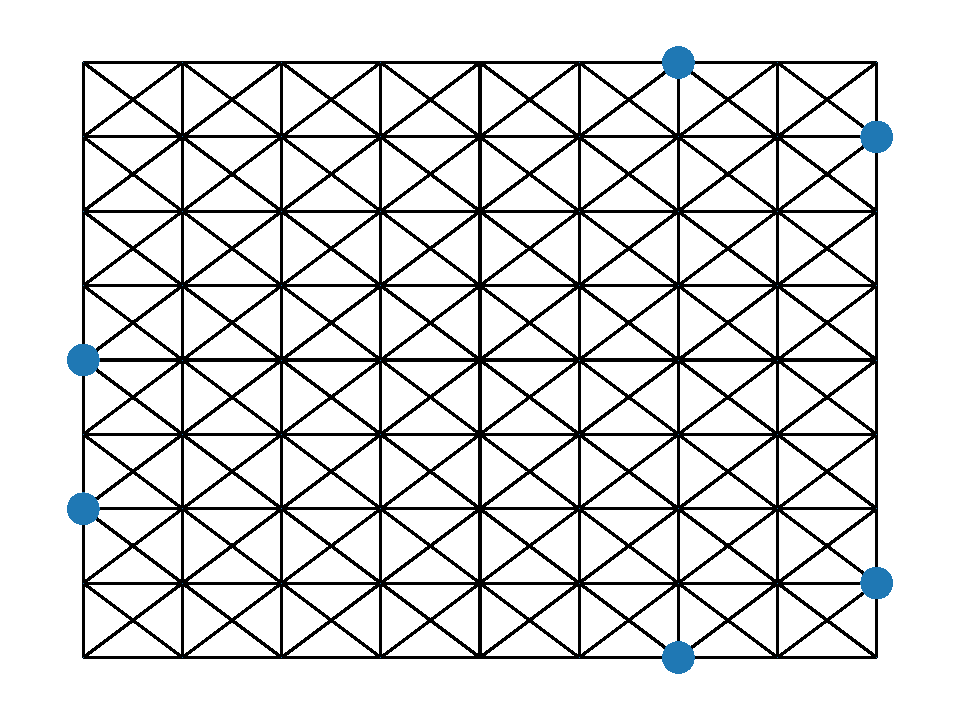
\includegraphics[width=\linewidth]{figures/algo_progress/default_graph_1-0.pdf}
        \caption{Generated grid-graph}
        \label{fig:def_1}
    \end{subfigure}
    \begin{subfigure}{0.32\linewidth}
        \centering
        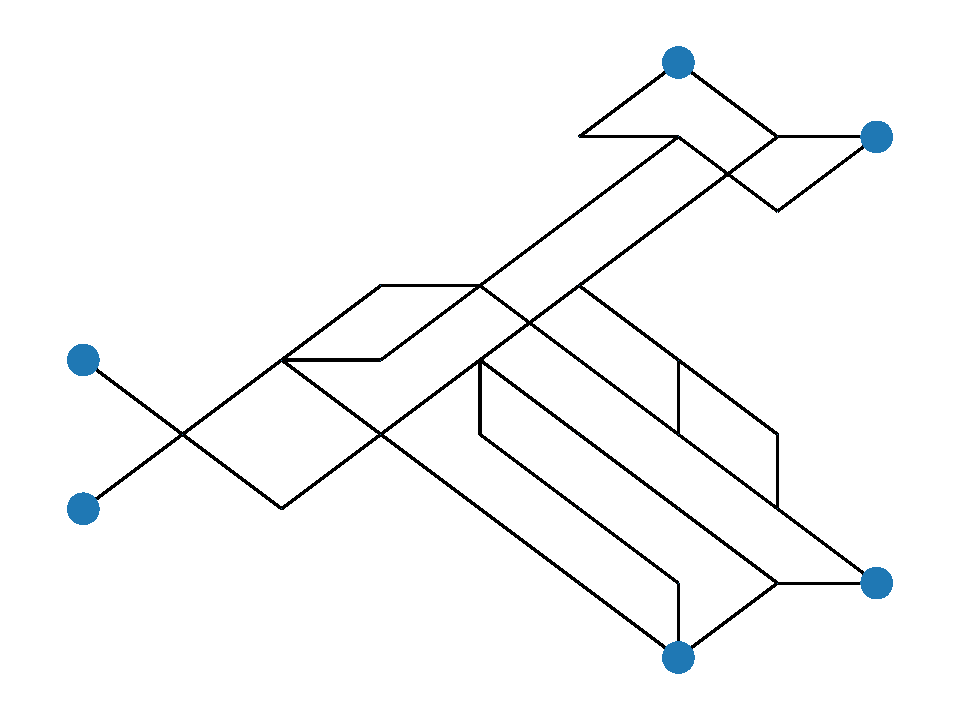
\includegraphics[width=\linewidth]{figures/algo_progress/default_graph_1-50.pdf}
        \caption{Grid after 50 iterations}
        \label{fig:def_2}
    \end{subfigure}
    \begin{subfigure}{0.32\linewidth}
        \centering
        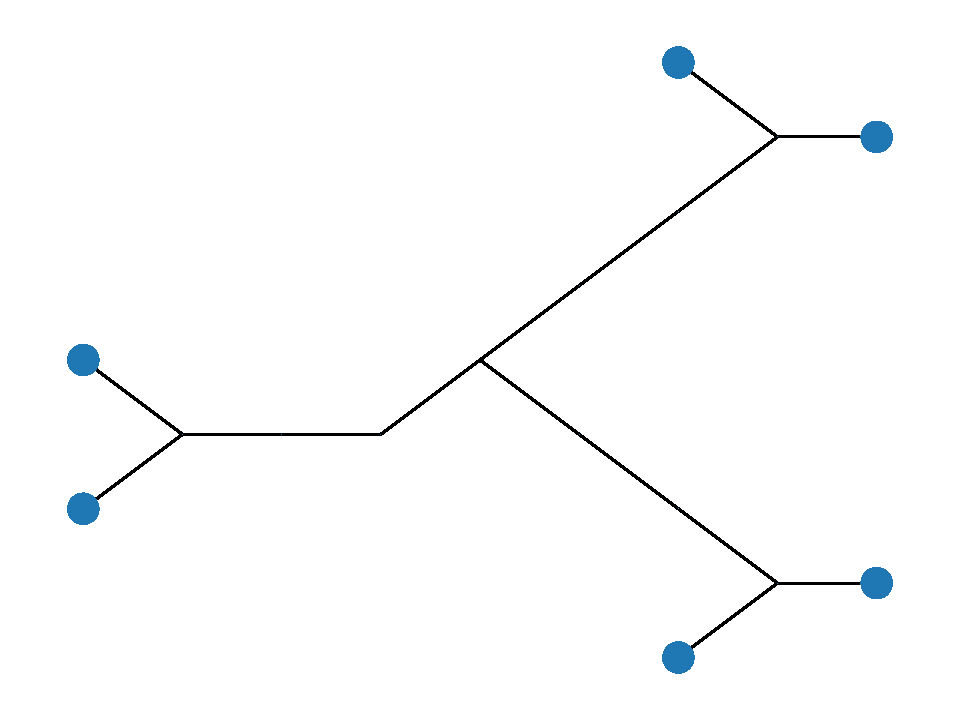
\includegraphics[width=\linewidth]{figures/algo_progress/without_clean_default.pdf}
        \caption{Finished calculation}
        \label{fig:def_3}
    \end{subfigure}
    \begin{subfigure}{0.32\linewidth}
        \centering
        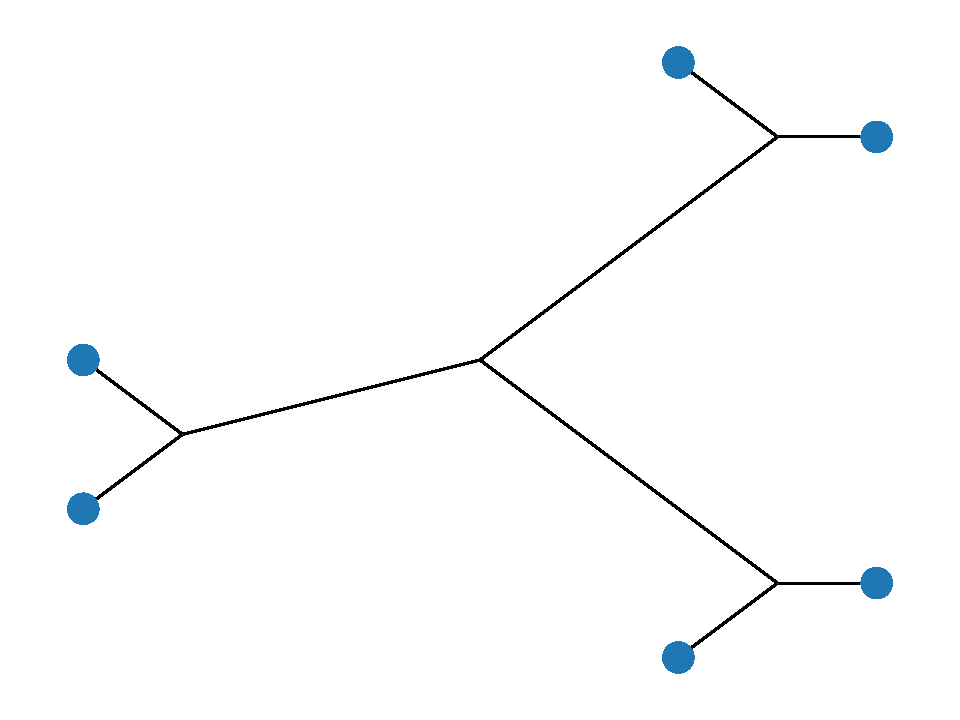
\includegraphics[width=\linewidth]{figures/algo_progress/unused_nodes_default.pdf}
        \caption{Removed unused nodes}
        \label{fig:def_4}
    \end{subfigure}
    \begin{subfigure}{0.32\linewidth}
        \centering
        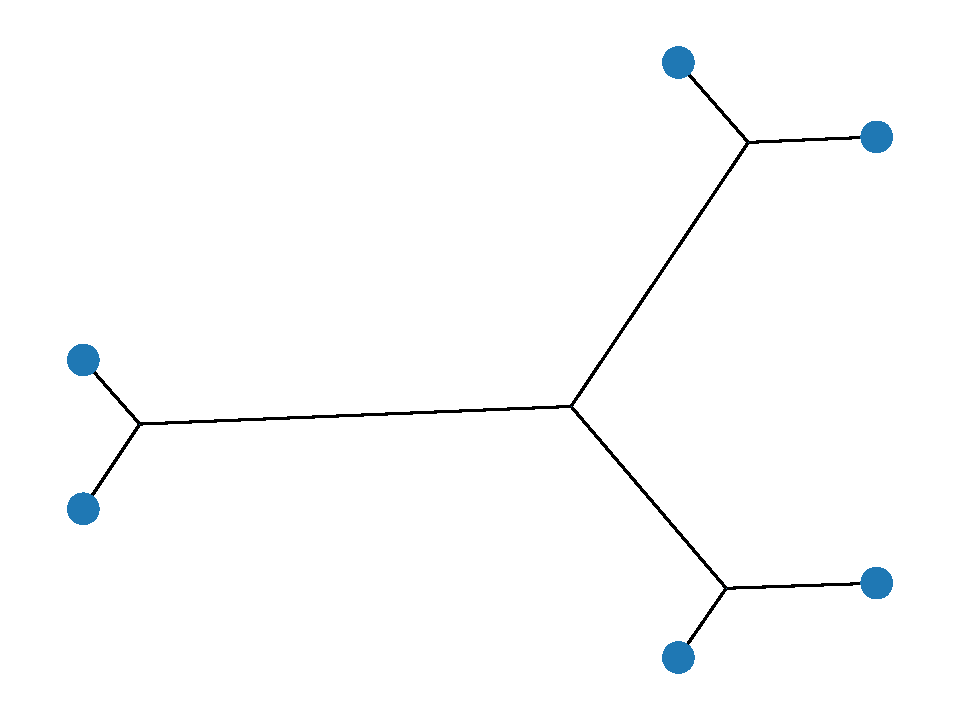
\includegraphics[width=\linewidth]{figures/algo_progress/fermat_default.pdf}
        \caption{Fermat point calculation}
        \label{fig:def_5}
    \end{subfigure}
  \caption{This figure visualizes the different steps our algorithm takes to reach a solution. \subref{fig:def_0} is the original graph as it is defined in the JSON file. Figure \subref{fig:def_1} is the grid graph built to calculate the Steiner points. \subref{fig:def_2} is the grid after 50 iterations; easy to spot is how the number of edges has shrunk. Figure \subref{fig:def_3} is the finished graph with the lowest cost. The solution from \subref{fig:def_3} still has unnecessary nodes, which are deleted by step \subref{fig:def_4}. The last step \subref{fig:def_5} is the Fermat point calculation that determines the position of the Steiner points.}
  \label{fig:default_combined}
\end{figure}

\section{Algorithm}
\label{sec:alogrithm}
We used a combination of the second and third approaches as our basis and expanded upon it. Our work is available on GitHub \cite{algortihm}.

% ************************************************************************
\begin{algorithm}
\caption{Physarium Steiner bundling}\label{psb_algorithm}
    \begin{algorithmic}
        \Require Graph $G = (V,E)$, with $V$ as terminals, viscosity value, initial flow
        
        \While {savedNetwork is None}
            \State Setup grid-environment $env$
            \State initialize edge conductivity
            \State calculate node and edge weights
            \For {outerIteration}
                \For {$edge \in edgeList$}
                    \State Initialize composite cost using \autoref{eqn:composite_cost_eqn}
                    \State Calculate the neighbor factor
                \EndFor
            
                \For {innerIteration}
                    \State Choose sink and source node using \autoref{eqn:probability_eqn}
                    \State Calculate pressure using \autoref{eqn:poisson_eqn}
        
                    \For {$edge \in edgeList$}
                        \State Calculate flux using \autoref{eqn:flux}
                        \State Update conductivities using \autoref{eqn:conductivity_update_eqn}
        
                        \If{edge conductivity < $\epsilon$}
                            \State Remove edge
                        \Else
                            \State Update edge conductivity
                            \State Calculate the neighbor factor
                        \EndIf
                    \EndFor
        
                    \If{Early inner iteration stop}
                        \For{$terminal \in terminalNodeList$}
                            \State Check terminal connections
                        \EndFor
        
                        \For{$edge \in edgeList$}
                            \State Calculate total edge cost
                            \State Check Steiner connections
                        \EndFor
                    \EndIf
                
                \EndFor
        
                \For{$edge \in edgeList$}
                    \State Calculate total edge cost
                    \State Check Steiner connections
                \EndFor
        
                \State \textbf{return} totalEdgeCost, steinerConnections
                
            \EndFor
        
            \If{toalEdgeCost $<$ currentEdgeCost}
                \State Current network becomes savedNetwork
            \EndIf
        
            \If{savedNetwork is None}
                \State innerIteration $*$ 1.5
                \State outerIteration $+$ number of cores $+$ 4
            \EndIf
            
        \EndWhile    
    \end{algorithmic}
\end{algorithm}
% ************************************************************************

%%%%%%%%%%%%%%%%%%%%%%%%%%%%%%%%%%%%%%%%%%%%%%%%%%%%%%%%%%%%%%%%%%%%%%%%

%%%%%%%%%%%%%%%%%%%%%%%%%%%%%%%%%%%%%%%%%%%%%%%%%%%%%%%%%%%%%%%%%%%%%%%%
\subsection{Building the Grid Graph}
\label{sec:grid_graph}
The first thing we did was build our grid graph generation, as the other papers did not mention how they got their grid graph. We calculated the dimensions of the graph by subtracting the minimal $x$ and $y$ values from the maximal values. The subtraction prevents unnecessary node creation if the graph does not begin at the origin of the coordinate system. 

In the next step, each node is connected to all nodes in a radius of $\sqrt{2}$. This means that a node in the center of the grid has eight connections, allowing for a more straightforward Steiner point calculation. With this method, we created the grid graph in \autoref{fig:def_1} from the original graph \autoref{fig:def_0}.

Not all graphs have node weights, so we set our weights and edge cost. The node weight is the sum of the euclidean distances between the node and each terminal. 

\begin{equation}
    \label{eqn:node_weights}
    w_i = \sum\limits_{j=0}^{|T|}  \sqrt{(x_{t_j} - x_i)^2 + (y_{t_j} - y_i)^2}
\end{equation}

The edge cost is the weights of its start and end node divided by the number of edges. 

\begin{equation}
    \label{eqn:edge_cost}
    c_{i,j} = \frac{w_i + w_j}{|E|}
\end{equation}
%%%%%%%%%%%%%%%%%%%%%%%%%%%%%%%%%%%%%%%%%%%%%%%%%%%%%%%%%%%%%%%%%%%%%%%%

%%%%%%%%%%%%%%%%%%%%%%%%%%%%%%%%%%%%%%%%%%%%%%%%%%%%%%%%%%%%%%%%%%%%%%%%
\subsection{Physarium Calculation}
\label{sec:physarium_calculation}
After the grid graph is created and the edges get their associated cost, the Physarium calculation can start. It begins by initializing the conductivity and the composite cost according to \autoref{eqn:conductivity_eqn} and \autoref{eqn:composite_cost_eqn}. 
In the next step, the sink node is chosen by \autoref{eqn:probability_eqn}, and the pressure is calculated with \autoref{eqn:poisson_eqn}. 
Next, the flux is calculated by \autoref{eqn:flux}, and the conductivity of each edge is updated using \autoref{eqn:conductivity_update_eqn}. If the conductivity is smaller than the threshold, it will be cut from the graph. In \autoref{fig:def_2} and \autoref{fig:def_3}, two iteration steps are illustrated, one after 50 iterations and the other at the end of the Physarium calculation.

These calculations continue until the iterations stop is reached. However, the graph can stabilize before implementing an early iteration stop if the graph does not change for several iteration steps. The exact number of steps is the number of edges in the grid graph before any calculations are performed. It also checks that each terminal has only one connection and that no node has more than three. The total edge cost is calculated and checked against the currently best-cost network. If the new cost is lower, the new network is saved, and the following calculation is executed until the outer iteration limit is reached. 
%%%%%%%%%%%%%%%%%%%%%%%%%%%%%%%%%%%%%%%%%%%%%%%%%%%%%%%%%%%%%%%%%%%%%%%%

%%%%%%%%%%%%%%%%%%%%%%%%%%%%%%%%%%%%%%%%%%%%%%%%%%%%%%%%%%%%%%%%%%%%%%%%
\section{Optimization}
\label{sec:optimization}

A significant part of our work was to optimize and test the algorithm as much as possible, as Sun et al. \cite{sun_fast_2016} only tried their algorithm with 100 vertices, and our goal was to solve at least a 25 x 25 grid in an acceptable amount of time.
The first step was, in addition to removing the edges, to remove all nodes that no longer had any connections to the rest of the grid, as they served no purpose. As in the next iteration step, they no longer influence the network. Other improvements include the integration of initialization of conductivity into the edge creation, a faster grid creation algorithm, and multi-threading of the main algorithm. 

Nevertheless, during our initial tests, we discovered that the outer and inner iteration limits are the main reason for the poor performance. They could be reduced significantly and still produce a good approximation. The first step we took was to implement an early iteration stop if there are no longer edges removed for several iterations. The number of iterations required for the stop is the number of edges in the graph at the start of the algorithm. We calculate a 10x10 grid graph from 18.843 seconds to 4 seconds with these optimizations.

Our algorithm runs in $O\left(T_0 \cdot \left(n \cdot e + T_i\left(n^3\right)\right)\right)$, where $n = |V|$ number of nodes, $e = |E|$ number of edges, $T_0$ the number of outer iterations and $T_i$ the number of inner iterations.
%%%%%%%%%%%%%%%%%%%%%%%%%%%%%%%%%%%%%%%%%%%%%%%%%%%%%%%%%%%%%%%%%%%%%%%%

\newpage

%%%%%%%%%%%%%%%%%%%%%%%%%%%%%%%%%%%%%%%%%%%%%%%%%%%%%%%%%%%%%%%%%%%%%%%%
\begin{figure}[H]
  \centering
  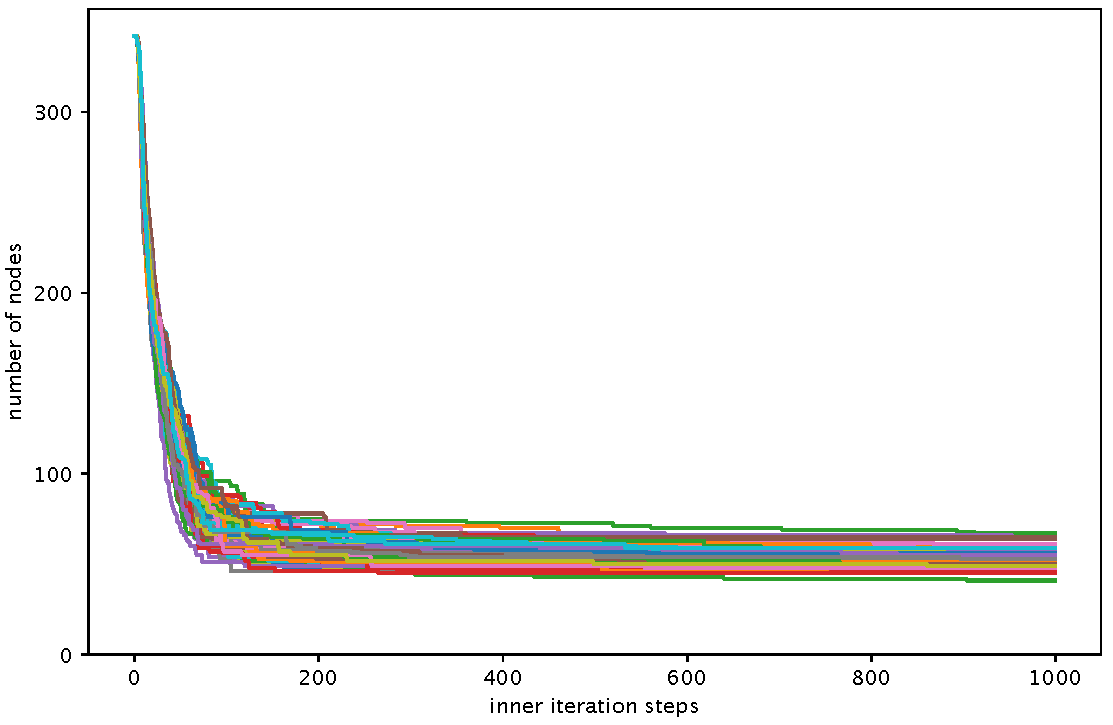
\includegraphics[width=1\linewidth]{figures/inner_iteration.pdf}
  \caption{The number of nodes in a 340 nodes test graph for the first 1000 inner iteration steps. The outer iteration was set to 100, meaning our algorithm calculated the test graph 100 times, and each line is one outer iteration. Easy to spot is the rapid decline in nodes in the first 100 iterations. This inside can be used for the optimal iteration bound.}
  \label{fig:inner_plots}
\end{figure}

\subsection{Inner Iteration Bound}
\label{sec:inner_iteration}

As one can see in \autoref{fig:inner_plots}, the most significant reduction of nodes takes place in the first 100 steps of the iteration. The size and structure of the graph have no impact on this result. We concluded that a lower bound for the inner iteration could improve the performance significantly, and the result would still be an acceptable Steiner tree approximation. As a sweet spot for the internal iteration limit, we found the inner iteration bound should be $|E|^{3}$. We added an exception for graphs where $|E|^{3}$ is smaller than 2000, as the iteration speed for those small graphs is fast either way, and the chance of a non-optimal Steiner tree is significantly reduced.
%%%%%%%%%%%%%%%%%%%%%%%%%%%%%%%%%%%%%%%%%%%%%%%%%%%%%%%%%%%%%%%%%%%%%%%%

%%%%%%%%%%%%%%%%%%%%%%%%%%%%%%%%%%%%%%%%%%%%%%%%%%%%%%%%%%%%%%%%%%%%%%%%
\begin{figure}[H]
  \centering
  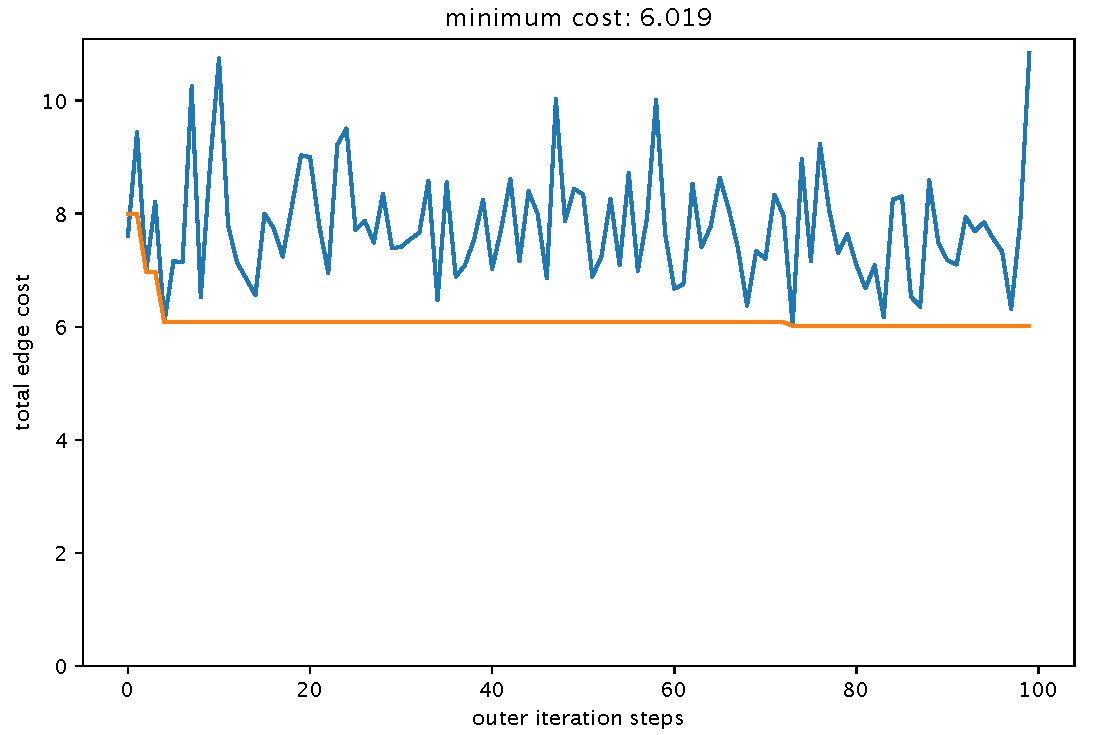
\includegraphics[width=1\linewidth]{figures/outer_iteration.pdf}
  \caption{This graph shows how the cost of the graph can reach a minimum early on and that it only improves slightly. The current minimum is displayed as the orange line, and the calculated minimum is the blue line.}
  \label{fig:outer_plots}
\end{figure}

\subsection{Outer Iteration Bound}
\label{sec:outer_iteration}

Initially, the number of outer iterations was determined by multiplying the x and y-axis. However, as the \autoref{fig:outer_plots} suggests, many external iterations are unnecessary. The algorithm only needs a few iterations to find a network shorter than the minimal spanning tree. From that point onward, the gains for running more iterations diminished rapidly as the length of the graph only shortened by a tiny amount. These gains are even further reduced by our post-processing method, which is discussed in the next section.
The number of outer iterations is the number of processing cores on the machine the algorithm is running. To ensure that the approximation calculated a good Steiner tree, we check if the total length is smaller than the minimal spanning tree. If that is not the case, we again start the outer iterations, only this time, we multiply the inner iteration bound by 1.5.
%%%%%%%%%%%%%%%%%%%%%%%%%%%%%%%%%%%%%%%%%%%%%%%%%%%%%%%%%%%%%%%%%%%%%%%%

%%%%%%%%%%%%%%%%%%%%%%%%%%%%%%%%%%%%%%%%%%%%%%%%%%%%%%%%%%%%%%%%%%%%%%%%
\section{Graph Cleaning and Post-Processing}
\label{sec:cleaning_and_processing}

% ************************************************************************
\begin{table*}[tb]
  \centering
  \setlength\tabcolsep{5pt} % adjust white space inside table
  \caption{
    \label{tab:cost}
    This table displays the network cost with the minimal spanning tree, the optimized approximation bound, and the approximation with high outer and inner iteration bounds. The time is for the lower approximation and the higher approximation. For the calculation, an Apple MacBook Air M1 was used.
  }  
  \begin{tabular}{c || c c c c c c}
    \toprule
     & \textbf{MST} & \textbf{low app.} & \textbf{high app.} & \textbf{ratio} & \multicolumn{2}{c}{\bfseries time} \\
     \hline
    3\_nodes & 2.000 & 1.337 & 1.337 & 1.000 & - & - \\
    5\_nodes & 4.000 & 2.314 & 2.314 & 1.000 & - & - \\
    9\_nodes & 8.000 & 5.155 & 4.962 & 1.039 & - & - \\
    default & 5.000 & 3.546 & 3.303 & 1.074 & - & - \\
    paper\_graph & 8.000 & 5.444 & 5.184 & 1.050 & - & - \\
    25x25\_10n\_30e & 5.000 & 4.254 & 4.032 & 1.055 & - & - \\
    10x10\_10n\_30e & 9.000 & 6.748 & 5.595 & 1.206 & - & - \\
    15x15\_15n\_30e & 14.000 & 13.272 & 11.987 & 1.107 & 25:39 & 1:57:33 \\
    15x15\_10n\_40e & 5.000 & 5.941 & 5.345 & 1.111 & 00:06 & 04:37 \\
    10x10\_10n\_30e & 5.000 & 6.230 & 5.755 & 1.083 & 00:03 & 03:08 \\
    \bottomrule
  \end{tabular}
\end{table*}
% ************************************************************************

When the graph calculations are finished, and a graph is found, the graph still needs to be cleaned, as there are still unnecessary nodes left, and the Steiner points are not at their correct position, as seen in \autoref{fig:def_3}.

So the first step is to remove unused nodes. The removal of the nodes is done by starting at the terminals or Steiner points and searching along the remaining edges for nodes that only have two connections until either a Steiner node or another terminal is reached. If the unused nodes are removed, the graph looks link \autoref{fig:def_4}.
The most important part of the post-processing is the calculation of the coordinates of the Steiner points. The computation works by utilizing the Fermat point calculation already mentioned in \autoref{sec:fermat_point}. As the points for the analysis can be Steiner points, we iterate through each point until the position does not change, and we archive a stable graph. An example of the Fermat point calculation can be seen in \autoref{fig:def_5}.

After post-processing, the approximation ratio we archived was 1.024, which indicates an excellent approximation quality. We calculated it by comparing our optimized approximation calculation against an approximation where we set the outer and inner iteration bounds to a value ten times as high. Our results for different synthetic graphs and calculation time can be seen in \autoref{tab:cost}.
%%%%%%%%%%%%%%%%%%%%%%%%%%%%%%%%%%%%%%%%%%%%%%%%%%%%%%%%%%%%%%%%%%%%%%%%

%%%%%%%%%%%%%%%%%%%%%%%%%%%%%%%%%%%%%%%%%%%%%%%%%%%%%%%%%%%%%%%%%%%%%%%%
\section{Path Visualisation}
\label{sec:path_visualisation}

\begin{figure}[t]
  \centering
  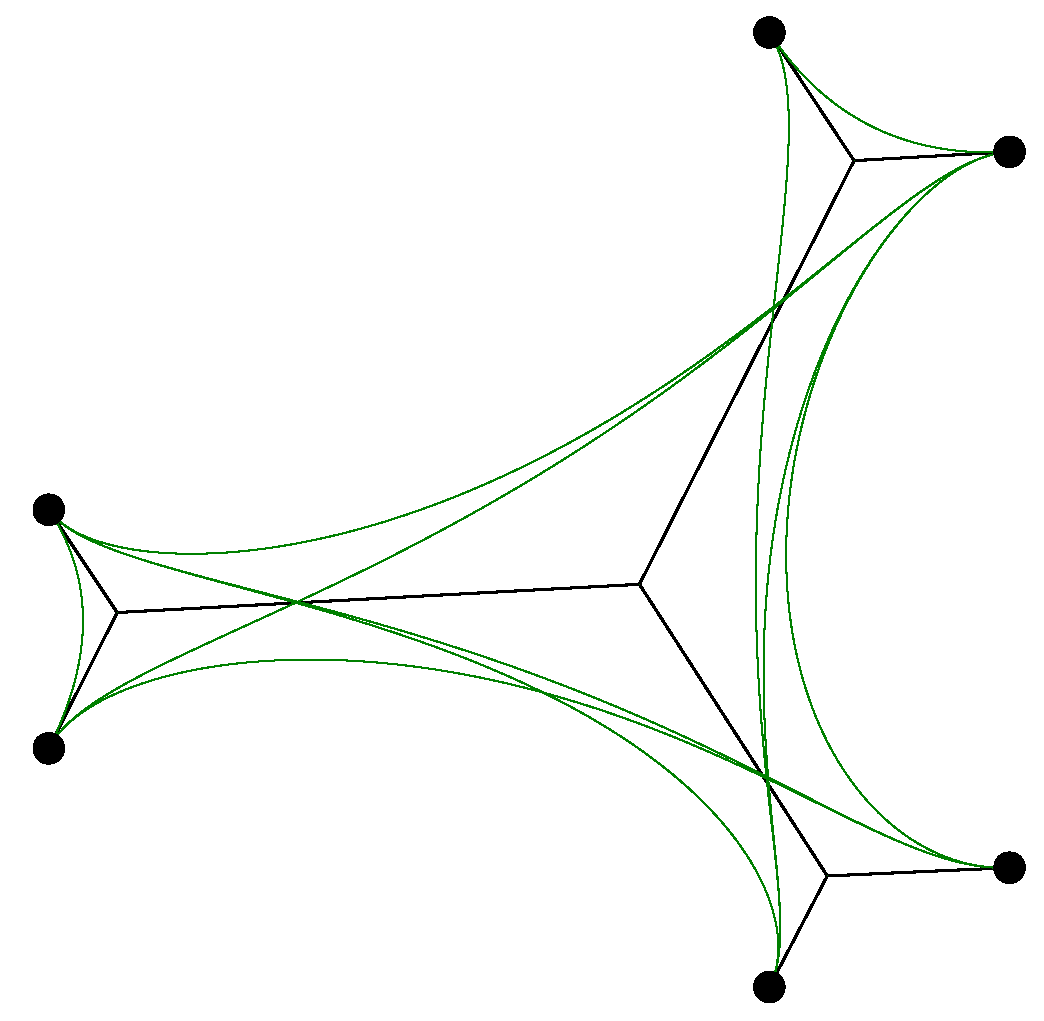
\includegraphics[width=0.6\linewidth]{figures/default_bezier+steiner.pdf}
  \caption{To better picture how the bundling works, we visualized the underlying Steiner tree and the B\'{e}zier curves in green. In the final plot, only the green edges will be visible.}
  \label{fig:default_bezier_steiner}
\end{figure}

After the post-processing cleaned the graph of unnecessary nodes and edges, only the approximated Steiner tree is left. The Steiner tree then routes the original paths along its edges. This skeletal structure gives us the ideal basis for bundling the actual paths. An example of the result can be seen in \autoref{fig:default_bezier_steiner}. The first bundling option we chose was to use the Steiner points as control points for a B\'{e}zier curve plot of the paths. This results in a bundle that is flexible in its representation and allows for a dynamic flow. In addition to the Steiner points as control points, we implemented a smoothing factor that enables the control points to be set on the edges of the tree. With each factor increase, the number of control points increased twofold.
%%%%%%%%%%%%%%%%%%%%%%%%%%%%%%%%%%%%%%%%%%%%%%%%%%%%%%%%%%%%%%%%%%%%%%%%

%%%%%%%%%%%%%%%%%%%%%%%%%%%%%%%%%%%%%%%%%%%%%%%%%%%%%%%%%%%%%%%%%%%%%%%%
\section{Graph Data and Experiments}
\label{sec:testing}

A big part of our work focused on testing and dialing the best parameters for a good approximation result. As our algorithm was still too slow for real-world graphs, we wrote a program to generate random graphs of any size and any possible combination of nodes and edges. This random graph generation enables us to test increasingly larger and more complex graphs starting from small 3x3 grid graphs up to 25x25 grid graphs. We discovered that the density of the graph significantly impacts the running time, which can even go so far that our algorithm can find no graph if the density is too high, as no Steiner tree can be created. This could be mitigated by increasing the resolution of the grid, but that would, on the other hand, impact the running time again.
We also tested alternative methods to reduce the number of nodes at the start of the approximation by running an initial calculation where the algorithm only calculates 10, 50, or 100 inner iterations. As the majority of node and edge deletions take place in these early iteration steps. Nevertheless, as our experiments have shown us, owning to the randomness of the terminal selection, it could happen that in these early stages, a crucial part of the graph network was deleted, and the following calculations could not archive a satisfactory result.
%%%%%%%%%%%%%%%%%%%%%%%%%%%%%%%%%%%%%%%%%%%%%%%%%%%%%%%%%%%%%%%%%%%%%%%%

  %!TEX root = ../Thesis.tex

%%%%%%%%%%%%%%%%%%%%%%%%%%%%%%%%%%%%%%%%%%%%%%%%%%%%%%%%%%%%%%%%%%%%%%%%
\chapter{Results}
\label{chap:Results}

The result of this thesis is a novel edge bundling algorithm that uses a Physarium Steiner tree calculation to build a structure that can then use to bundle the paths. As mentioned in \autoref{sec:testing}, we generated the graphs that we then compared to the Edge-Path bundling approach by Wallinger et al. \cite{wallinger_edge-path_2022}, and the Winding Roads method by Lambert et al. \cite{lambert_winding_2010}, as these have made their algorithms readily available, we already have a good understanding of how they work, and they are representative of a method with an underlying structure and one without one.

%%%%%%%%%%%%%%%%%%%%%%%%%%%%%%%%%%%%%%%%%%%%%%%%%%%%%%%%%%%%%%%%%%%%%%%%

\section{Quality Metrics}
%%%%%%%%%%%%%%%%%%%%%%%%%%%%%%%%%%%%%%%%%%%%%%%%%%%%%%%%%%%%%%%%%%%%%%%%

\begin{figure}[t]
    \centering
    \begin{subfigure}{0.3\linewidth}
        \centering
        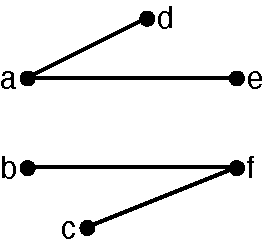
\includegraphics[width=0.9\linewidth]{figures/amb_value/0_amb_value.pdf}
        \caption{Straight-line graph}
        \label{fig:amb_value_0}
    \end{subfigure}
    \begin{subfigure}{0.3\linewidth}
        \centering
        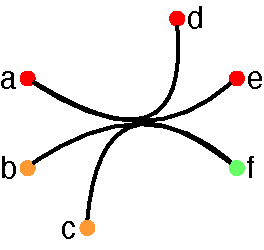
\includegraphics[width=0.9\linewidth]{figures/amb_value/1_amb_value.pdf}
        \caption{Bundled graph}
        \label{fig:amb_value_1}
    \end{subfigure}
  \caption{\subref{fig:amb_value_1} is a possible bundle of \subref{fig:amb_value_0}. In \subref{fig:amb_value_1}, all red nodes are false neighbors $N_{\Gamma}^f$ for the b node, and all yellow nodes are false neighbors $N_{\Gamma}^f$ for f. \cite{Straub2022}}
  \label{fig:ambiguity_2}
\end{figure}

To compare those three algorithms, we utilize the three quality metrics provided by Wallinger et al. \cite{wallinger_edge-path_2022} and modify them according to our needs. 
The ink reduction $ink(I)$ reveals how many edges were bundled and how much the bundling reduced the clutter by counting the non-white pixels in a plot. $I_B$ is the bundled plot and $I_O$ the original plot.

\begin{equation}
    ink(I)=\frac{\sum_{i=1}^m \sum_{j=1}^n I_B(i,j)}{\sum_{i=1}^m \sum_{j=1}^n I_O(i,j)}
\end{equation}

The bundling reduced clutter inside the graph if the number of non-white pixels shrank.
The next metric, $dist(\Gamma)$, tells if the bundled edges make a long detour or remain close to the Euclidean distance. Suppose they had a long detour that would make adjacencies harder to read. 

\begin{equation}
    dist(\Gamma)= \sum_{(u,v)\in E} \frac{d_{\Gamma}(u,v)}{||u-v||}
\end{equation}

The distortion value is calculated by dividing the length of the sum of the edges of the bundled graph by that of the original.
The ambiguity metric $amb(\Gamma)$ reveals the perceivable false connections within the bundled graph.

\begin{equation}
    amb(\Gamma)=\frac{\sum_{v \in V} \sum_{e=(v,w)\in E} |N_{\Gamma}^f(v,e)|}{\sum_{v \in V} \sum_{e=(v,w)\in E} |N_{\Gamma}(v,e)|}
\end{equation}

To calculate this, we divide all false neighbors by all possible neighbors. $N_{\Gamma}$ is the number of reachable neighbors from a node $x$ with edge $e$. $N_{\Gamma}^f$ are all false neighbours. \autoref{fig:ambiguity_2} is an example of the relationship between true and false neighbors.
A connection is ambiguous if two edges intersect with a slight angle or the distance between them is too small to distinguish them.
%%%%%%%%%%%%%%%%%%%%%%%%%%%%%%%%%%%%%%%%%%%%%%%%%%%%%%%%%%%%%%%%%%%%%%%%
% ************************************************************************
\begin{table*}[tb]
  \centering
  \setlength\tabcolsep{5pt} % adjust white space inside table
  \caption{
    \label{tab:quality}
    The table displays the quality metrics scores for our four synthetic data graphs. The bundled drawings for the \textbf{default} graph are displayed here \autoref{fig:default_bezier_steiner}, for the \textbf{10x10} graph here \autoref{fig:10x10_figure}, for the \textbf{15x15} graph here \autoref{fig:15x15_figure} and the \textbf{25x25} graph here \autoref{fig:25x25_figure}.
  }  
  \begin{tabular}{p{0.045\linewidth} || p{0.045\linewidth} p{0.045\linewidth} p{0.055\linewidth} | p{0.045\linewidth} p{0.045\linewidth} p{0.055\linewidth} | p{0.045\linewidth} p{0.045\linewidth} p{0.055\linewidth} | p{0.045\linewidth} p{0.045\linewidth} p{0.055\linewidth}}
    \toprule
     & \multicolumn{3}{c|}{\bfseries default} & \multicolumn{3}{c|}{\bfseries 10x10\_10n\_30e} & \multicolumn{3}{c|}{\bfseries 15x15\_10n\_40e} & \multicolumn{3}{c}{\bfseries 25x25\_10n\_30e}\\
     & $ink$ & $dist$ & $amb$ & $ink$ & $dist$ & $amb$ & $ink$ & $dist$ & $amb$ & $ink$ & $dist$ & $amb$ \\
    \midrule
    Org & 1.000 & 1.000 & 0.000 & 1.000 & 1.000 & 0.035 & 1.000 & 1.00 & 0.037 & 1.00 & 1.00 & 0.100 \\
    WR & 0.686 & \textbf{0.985} & \textbf{0.000} & 0.677 & \textbf{1.055} & 0.070 & 0.700 & \textbf{1.017} & \textbf{0.062} & \textbf{0.643} & \textbf{1.001} & \textbf{0.033} \\
    EPB & 1.553 & 1.321 & \textbf{0.000} & 1.368 & 1.169 & \textbf{0.053} & 1.167 & 1.179 & 0.075 & 1.513 & 1.177 & 0.100 \\
    PSB & \textbf{0.685} & 0.955 & \textbf{0.000} & \textbf{0.613} & 1.060 & 0.122 & \textbf{0.562} & 1.126 & 0.075 & 0.728 & 1.191 & 0.133 \\
    \bottomrule
  \end{tabular}
\end{table*}
% ************************************************************************

\begin{figure}[H]
    \begin{subfigure}{0.5\linewidth}
        \centering
        \includegraphics[width=\linewidth]{figures/10x10/original_10x10_10n_30e.png}
        \caption{Straight-line graph}
        \label{fig:original_10x10}
    \end{subfigure}
    \begin{subfigure}{0.5\linewidth}
        \centering
        \includegraphics[width=\linewidth]{figures/10x10/wr_10x10_10n_30e.png}
        \caption{Winding Roads}
        \label{fig:wr_10x10}
    \end{subfigure}
    \begin{subfigure}{0.5\linewidth}
        \centering
        \includegraphics[width=\linewidth]{figures/10x10/epb_10x10_10n_30e.png}
        \caption{Edge-Path bundling}
        \label{fig:epb_10x10}
    \end{subfigure}
    \begin{subfigure}{0.5\linewidth}
        \centering
        \includegraphics[width=\linewidth]{figures/10x10/10x10_10n_30e_12-1000.png}
        \caption{Physarium Steiner bundling}
        \label{fig:10x10}
    \end{subfigure}
  \caption{These are example solutions for a 10x10 grid graph. The original straight-line graph is presented in \subref{fig:original_10x10}. With these plots, the strike bundling of our method in \subref{fig:10x10} can be seen.
  As all three algorithms use different techniques to plot the graph, slight visual variations may be noticeable.}
  \label{fig:10x10_figure}
\end{figure}

\begin{figure}[H]
    \begin{subfigure}{0.5\linewidth}
        \centering
        \includegraphics[width=\linewidth]{figures/15x15/original_15x15_10n_40e.png}
        \caption{Straight-line graph}
        \label{fig:original_15x15}
    \end{subfigure}
    \begin{subfigure}{0.5\linewidth}
        \centering
        \includegraphics[width=\linewidth]{figures/15x15/wr_15x15_10n_40e.png}
        \caption{Winding Roads}
        \label{fig:wr_15x15}
    \end{subfigure}
    \begin{subfigure}{0.5\linewidth}
        \centering
        \includegraphics[width=\linewidth]{figures/15x15/epb_15x15_10n_40e.png}
        \caption{Edge-Path bundling}
        \label{fig:epb_15x15}
    \end{subfigure}
    \begin{subfigure}{0.5\linewidth}
        \centering
        \includegraphics[width=\linewidth]{figures/15x15/15x15_10n_40e_12-1000.png}
        \caption{Physarium Steiner bundling}
        \label{fig:15x15}
    \end{subfigure}
  \caption{These are example solutions for a 15x15 grid graph. The original straight-line graph is presented in \subref{fig:original_15x15}. Interestingly to us is that \subref{fig:epb_15x15} and \subref{fig:15x15} look similar in regards to their ink reduction, but their metrics in \autoref{tab:quality} do not confirm this observation. This is the only plot out of the three examples where the Physarium Steiner bundling looks similar to one of the other approaches in this chase Edge-Path bundling.
  As all three algorithms use different techniques to plot the graph, slight visual variations may be noticeable.}
  \label{fig:15x15_figure}
\end{figure}

\begin{figure}[H]
    \begin{subfigure}{0.5\linewidth}
        \centering
        \includegraphics[width=\linewidth]{figures/25x25/original_25x25_10n_30e.png}
        \caption{Straight-line graph}
        \label{fig:original_25x25}
    \end{subfigure}
    \begin{subfigure}{0.5\linewidth}
        \centering
        \includegraphics[width=\linewidth]{figures/25x25/wr_25x25_10n_30e_graph.png}
        \caption{Winding Roads}
        \label{fig:wr_25x25}
    \end{subfigure}
    \begin{subfigure}{0.5\linewidth}
        \centering
        \includegraphics[width=\linewidth]{figures/25x25/epb_25x25_10n_30e_graph.png}
        \caption{Edge-Path bundling}
        \label{fig:epb_25x25}
    \end{subfigure}
    \begin{subfigure}{0.5\linewidth}
        \centering
        \includegraphics[width=\linewidth]{figures/25x25/25x25_10n_30e_12-1000.png}
        \caption{Physarium Steiner bundling}
        \label{fig:25x25}
    \end{subfigure}
  \caption{These are example solutions for a 25x25 grid graph. The original straight-line graph is presented in \subref{fig:original_25x25}. With these plots, it is easy to spot the striker bundling approach of \subref{fig:25x25}. All long edges that remain relatively straight and original are merged into the main bundle in the middle.
  As all three algorithms use different techniques to plot the graph, slight visual variations may be noticeable.}
  \label{fig:25x25_figure}
\end{figure}

\section{Comparison}
\label{sec:comparison}

As mentioned in \autoref{sec:testing}, our algorithm is too slow to solve real-world graphs, and we, therefore, rely on synthetic data we generated. The default dataset has six nodes and was the graph we tested new features throughout the testing phase, as it is fast to calculate, and the resulting Steiner tree is known. It is also the only graph that is not randomly generated. The others get increasingly complex and grow in size. The increasing complexity was done to test the limits and see the behavior of the calculation \autoref{tab:quality}. 

\subsection{Ink Reduction}
\label{sec:ink_reduction}
Logically the ink reduction of the straight-line graph is one. Edge path bundling performs the worst in this category as it uses the shortest edges of the existing path network and a B\'{e}zier curve to visualize the longest paths. Winding Roads and our approach have a much higher degree of bundling, as both use an underlying structure to bundle. That the Physarium Steiner bundling comes out on top is to be expected, as it has a smaller frame to work with. The scores also fit the appearance of \autoref{fig:10x10}, \autoref{fig:15x15} and \autoref{fig:25x25}.

\subsection{Distortion}
\label{sec:distortion}
The distortion on a straight-line graph is, by definition, one. With this metric, the results are much closer, and Winding roads has the least distorted bundling. We observe that the distortion value of our approach is linked to the graph size; the larger the graph, the higher the distortion value. The high distortion value means that the greater the graph gets, the longer the detours of the paths must be, compared to their original counterparts. The longer detours exist because all paths must use the Steiner tree for their routing and if the graph increases in size, the detour through the Steiner tree becomes more significant than the direct path.

\subsection{Ambiguity}
\label{sec:ambiguity}
As even straight-line graphs can have ambiguities, it is to be expected that a low ambiguity value is present. Both Winding Roads and Edge Path bundling have only a slightly larger ambiguity value than the straight-line graph. These are caused by edge crossings which a shallow crossing angle. On the other hand, our approach consistently has the most ambiguities as the proximity of paths causes them. This results in a compact graph whose side effect is that it is more challenging to follow paths.
%%%%%%%%%%%%%%%%%%%%%%%%%%%%%%%%%%%%%%%%%%%%%%%%%%%%%%%%%%%%%%%%%%%%%%%%


  %!TEX root = ../Thesis.tex

%%%%%%%%%%%%%%%%%%%%%%%%%%%%%%%%%%%%%%%%%%%%%%%%%%%%%%%%%%%%%%%%%%%%%%%%
\chapter{Discussion and Limitations}
\label{sec:discussion}

Our Physarium Steiner bundling can bundle a graph very aggressively to reveal its overall structure and deduce what region might be of particular interest. A side effect of this aggressive bundling is that some parts of the graph become more ambiguous, particularly parts where the Steiner tree only has one connecting edge. On the other hand, the area around each outer node has a low ambiguity, and it is possible to distinguish each path. To mitigate those issues, a technique like Edgelens \cite{wong_edgelens_2003} could be used in those high-density regions. 

The mathematical structure of our approach makes it easy to anticipate the outcome, as paths can only follow the predetermined route. This might help with anticipating choke points where specific paths connect. These use cases are currently only theoretical, as we only have very little data to test our algorithm. As we already mentioned in \autoref{sec:distortion}, an increase in the distortion value is linked to a larger graph size. This could become a problem if we bundled real-world graphs, as they are many times larger. The distortion might be so severe that it would be impossible to distinguish paths. A possible solution would be to relax the bundling strength, as currently, all paths have to use the Steiner points. Instead, orthogonal to the Steiner points, other points could be created and subsequently used as alternative routing points. This would reduce the path density at the Steiner point. 

Larger graph data might also impact the ambiguity value, as more paths would be routed along the Steiner points. This could lead to significant edge-edge overlaps. However, our limited test data shows that the ambiguity does not change in the same way as the distortion changes when the size of the graph increases. It, therefore, remains to be seen how this algorithm performs for large graphs. 

Another significant shortcoming of this method is most definitely the performance. Despite the considerable time spent optimizing our algorithm, we could not improve the performance to a point where large, real-world datasets could be calculated. That not only limits the usefulness of a graph bundling algorithm but also severely limits the credibility of our comparison. Potential solutions for this problem are debated below.
%%%%%%%%%%%%%%%%%%%%%%%%%%%%%%%%%%%%%%%%%%%%%%%%%%%%%%%%%%%%%%%%%%%%%%%% 
  %!TEX root = ../Thesis.tex

%%%%%%%%%%%%%%%%%%%%%%%%%%%%%%%%%%%%%%%%%%%%%%%%%%%%%%%%%%%%%%%%%%%%%%%%
\chapter{Conclusion}
\label{sec:conclusion}

This work introduced a novel edge bundling technique based on a Physarium approximation of a Steiner tree. This Steiner tree is then used as a routing structure for graph paths. We evaluated and compared our algorithm using the quality metrics: ink reduction, distortion, and ambiguity. These metrics are computed on graph drawings of synthetic data we generated for testing pursues. The resulting illustrations consist of dense graphs that reduce node-edge overlaps, make reading easier, and make it more straightforward to spot areas of interest. Our algorithm has a worst-case complexity of $O\left(T_0 \cdot \left(n \cdot e + T_i\left(n^3\right)\right)\right)$ which is enough for small-scale synthetic graphs, but not enough to be used with real-world data, mainly because graph bundling becomes necessary if the graph data it too large to comprehend. 

The metrics comparison showed us that our approach has a reasonable degree of bundling and outperforms the other two techniques. This, however, comes at the cost of distortion and ambiguity. Nevertheless, the excellent ink reduction value is a promising sign that with a better approximation algorithm, our approach could be used to declutter graphs and isolate regions of interest. 

For us, future work could lead in two directions. The first would be to improve performance by using a GPU-based implementation to solve the matrices or abandoning the Physarium approximation and instead employ GeoSteiner \cite{winter_euclidean_1997}, or even better SCIP-Jack \cite{RehfeldtKoch2023} for a fast Steiner tree approximation. The other direction would be to utilize the Physarium-inspired approach to a Euclidean Steiner tree by Hsu \cite{hsu_physarum-inspired_2022}. With this, it should be possible to bundle real-world graph data.

To conclude: Our approach suffers from significant drawbacks caused by the slow approximation calculation, which hindered us from testing real-world graph data and, in turn, evaluating the usefulness of our method. Unfortunately, we discovered too late that our optimizations could not improve the approximation enough to become functional. 
Nevertheless, we still think it is a promising approach that could become feasible by utilizing the above-mentioned future work. 
%%%%%%%%%%%%%%%%%%%%%%%%%%%%%%%%%%%%%%%%%%%%%%%%%%%%%%%%%%%%%%%%%%%%%%%%

% This ensures that the subsequent sections are being included as root
% items in the bookmark structure of your PDF reader.
\bookmarksetup{startatroot} 
\backmatter
  
  \printbibliography
  
\end{document}